\chapter{Use cases of interest}
\label{chapter:use_cases}
%\todo{EB: titolo un po' troppo anonimo. Anche se non mi viene in mente niente. ``Use cases of interest''?}
In this chapter, the focus is to present two distinct projects, among several I have followed during my time at Zensor, highlighting the many useful elements covered in the previous three. % chapters
Therefore, it is logically divided into two parts:
\begin{enumerate}
    \item A discussion of a use scenario in an industrial environment, aimed at improving the production process and reducing downtime.
    \item A report on an energy monitoring project to reduce overall energy consumption and improve sustainability.
\end{enumerate}

% \todo{DG: Intro}

\section{Analyze blade grinder vibration}
% \todo{EB: si pu\`o dire la compagnia. Prima ci vuole una breve intro del task. E poi ci dirai quanto \`e stato difficile, etc.}
% Meglio?
In this section, we discuss how to improve an existing industrial machine, needed for blade production.
The three years old, installation has a high number of standstills (unplanned stop) with a strong impact on sales.
Furthermore, the excessive amount of vibrations on the machine has negative effect on quality of the cut, invalidating quality test results.
% I'd like to talk you about %% troppo informale
%\todo{EB: Continuare una frase cos\`i ``The full understanding of context of the problem demostrated to be crucial to...'' La frase corrente \`e troppo colloquiale}

We are also going to illustrate some difficulties encountered in vibration analysis and correlated problems, where 
the full understanding of problem's context demonstrated to be crucial.
Despite the lack of precise operational data, counter-intuitive results, the initial report was successful and helped to strengthen the methodology for further analysis.

\subsection{Initial Hypothesis}
\paragraph{Context Introduction}
\begin{figure}[ht]
    \begin{subfigure}{\textwidth}
        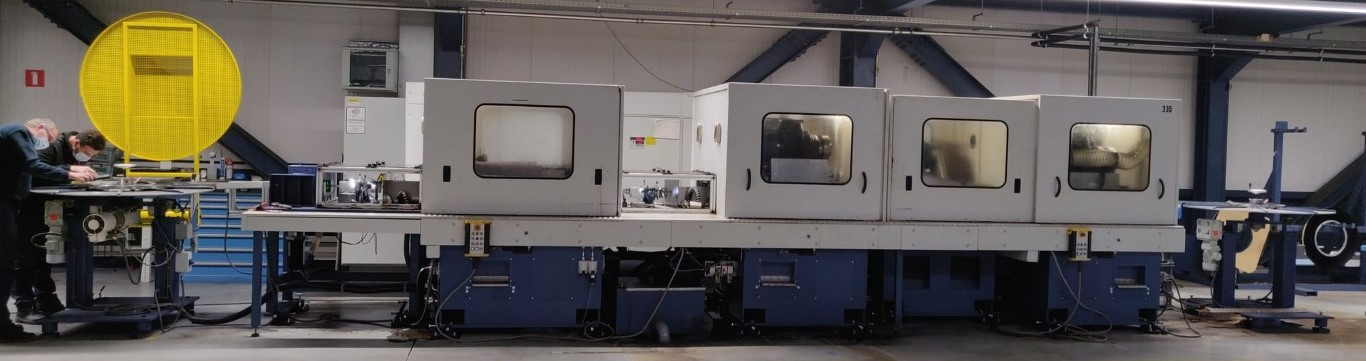
\includegraphics[width=\linewidth]{stumabo/installation/line_photo.jpg}
        \caption{Line overview: side view}
        \label{fig:line_overview}
    \end{subfigure}
    \begin{subfigure}{\textwidth}
        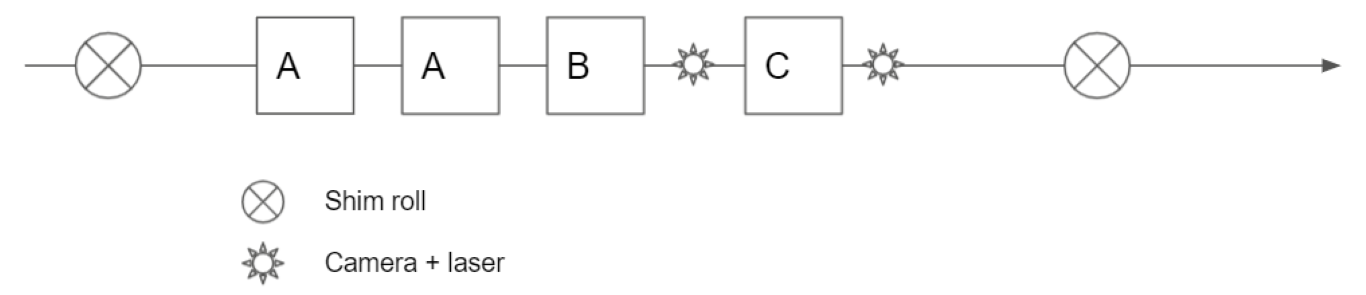
\includegraphics[width=\linewidth]{stumabo/installation/line_schematics.png}
        \caption{Line motor schematics}
        \label{fig:line_schematics}
    \end{subfigure}
    \caption{Stumabo's blade production line covered by this project}
    \label{fig:stumabo_prod_line}
\end{figure}
The subject of this monitoring operation is a blade-cutting machine line.
As shown in Figure~\ref{fig:stumabo_prod_line} there are four different stations (\subref{fig:line_overview}). Each of them has one or two motors type ${A,B,C}$ (\subref{fig:line_schematics}).
Each station has grinding stones to sharpen a blade, which is one long strip of steel passing through all the machines.
To perform their grinding task, the stones turn around their axe sharpening the steel blade, each machine in its own way.
% \todo{DG: dare definizione di campagna ad hoc? EB: questa non l'ho capita}

\paragraph{Client} Stumabo International, a manufacturer of precision blades for the food processing industry, produces several million blades per year, 
and it is known in the industry for their progressive industrial potato cutting solutions, and innovative shapes produced through hydro-cutting systems.
Stumabo also uses their knowledge to integrate the best blade in the FAM industrial mechanical cutters~\cite{Misc:stumabo_en_website}.

\subsection{Goal(s), purpose \& critical factors}
The project started in conjunction with the beginning of the internship (Oct-Nov 2021), and I had the pleasure of contributing in its early stages.
The main objective was to produce an \textit{ad-hoc}\footnote{It is usually produced only once, is more visual than a static report and, once completed, is shared with a smaller audience.} 
analysis report, that could answer specific business questions.
Unfortunately my practice ended before the second, more substantial monitoring phase of the project began, scheduled to be April 2022.
Let's see what the goals are in the long and short term and then exploring the latter.
\paragraph{Long term: project lifecycle}
\begin{itemize}
    \item[$\circledcirc$] Increase production quality through the use of continuous data analysis.
    \item[$\circledcirc$] Avoid unplanned standstill (downtime) by preventing critical component failures.
    \item[$\circledcirc$] Extends the life of machines and installation through \acl{PdM} and \acl{cm} (see Section \ref{section:maintenance})
\end{itemize}
\paragraph{Short term: \textit{ad-hoc} campaign}
\begin{itemize}
    \item[$\circledcirc$] Is  it possible to identify a strong impact of the turning of the grindstones? Perhaps a possible imbalance?
    \item[$\circledcirc$] As a general insight, do we have indication that something is causing strong vibration?
    \item[$\circledcirc$] Lastly, as preliminary path for the second stage, the \ac{CtM}, which key elements we should focus on? 
    \todo{EB: questo punto non l'ho capito, DG: meglio?}
\end{itemize}

\subsection{Project description by phases}
\begin{figure}[ht]
    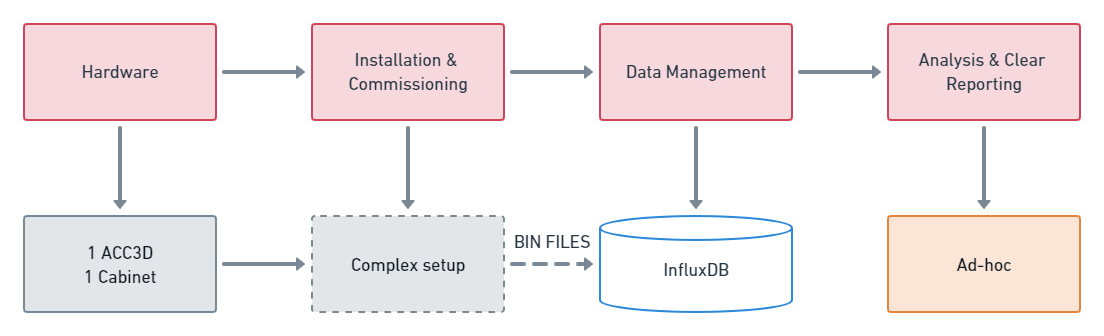
\includegraphics[width=\textwidth]{stumabo/21022_STU.png}
    \caption{Core Stages of this (full) project}
    \label{fig:stumabo_stages}
\end{figure}
As we saw earlier in Section~\ref{section:zensor_approach}, we can have two types of projects, \textit{full} and \textit{light}.
This one belongs to full or ``complete'' class, with some intense engineering (hardware \& installation) phases.  
% \todo{EB: ricordare cosa vuol dire un ``complete one' e troppo informale ``as the reader will have already guessed''.' EB: ci ho anche capito poco.}
\todo{Perch\'e less complex than big project? 
DG: perchè è una campagna di preparazione inziale.} \\
\todo{E cosa \`e un ``big'' project? big confonde, meglio full.
Magari era scrtto prima. Ma bene sia ricordarlo che aggiungere riferimento a ``prima'' DG: il riferimento era già presente ad inizio paragrafo, ne aggiungo un' altro?}

However, since this is a preparation (\textit{ad-hoc}) campaign, as mentioned earlier, it will have less complexity than a regular \textit{full} project.
To summarize it in one formula, given three variables ($f$ull, $l$ight, $s$tumabo) and ``complexity'' function $O(x)$ is true that $\forall f,l| O(l) \leq O(s) \leq O(f)$.
My contribution was to help with the analysis phase, but it's important to emphasize how the first three phases went, because they will have serious implications for data development and analysis.
\paragraph{Hardware} 
\begin{figure}[ht]
    \begin{subfigure}{0.33\textwidth}
        \centering
        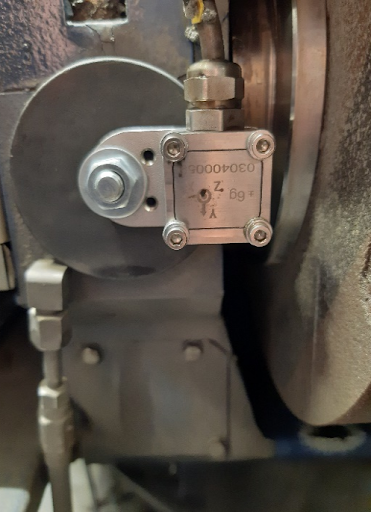
\includegraphics[height=\linewidth]{stumabo/installation/acc_station_1_blue.png}
        \caption{Installation photo}
        \label{fig:s1b_foto}
    \end{subfigure}
    \begin{subfigure}{0.33\textwidth}
        \centering
        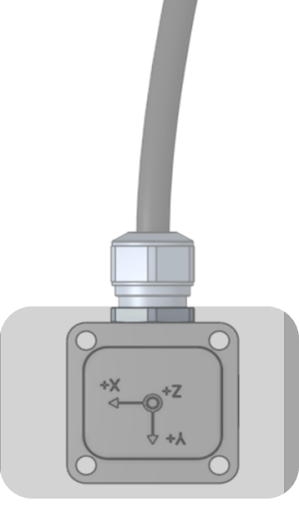
\includegraphics[height=\linewidth]{stumabo/installation/acc_render.png}
        \caption{CAD render}
        \label{fig:s1b_render}
    \end{subfigure}
    \begin{subfigure}{0.32\textwidth}
        \centering
        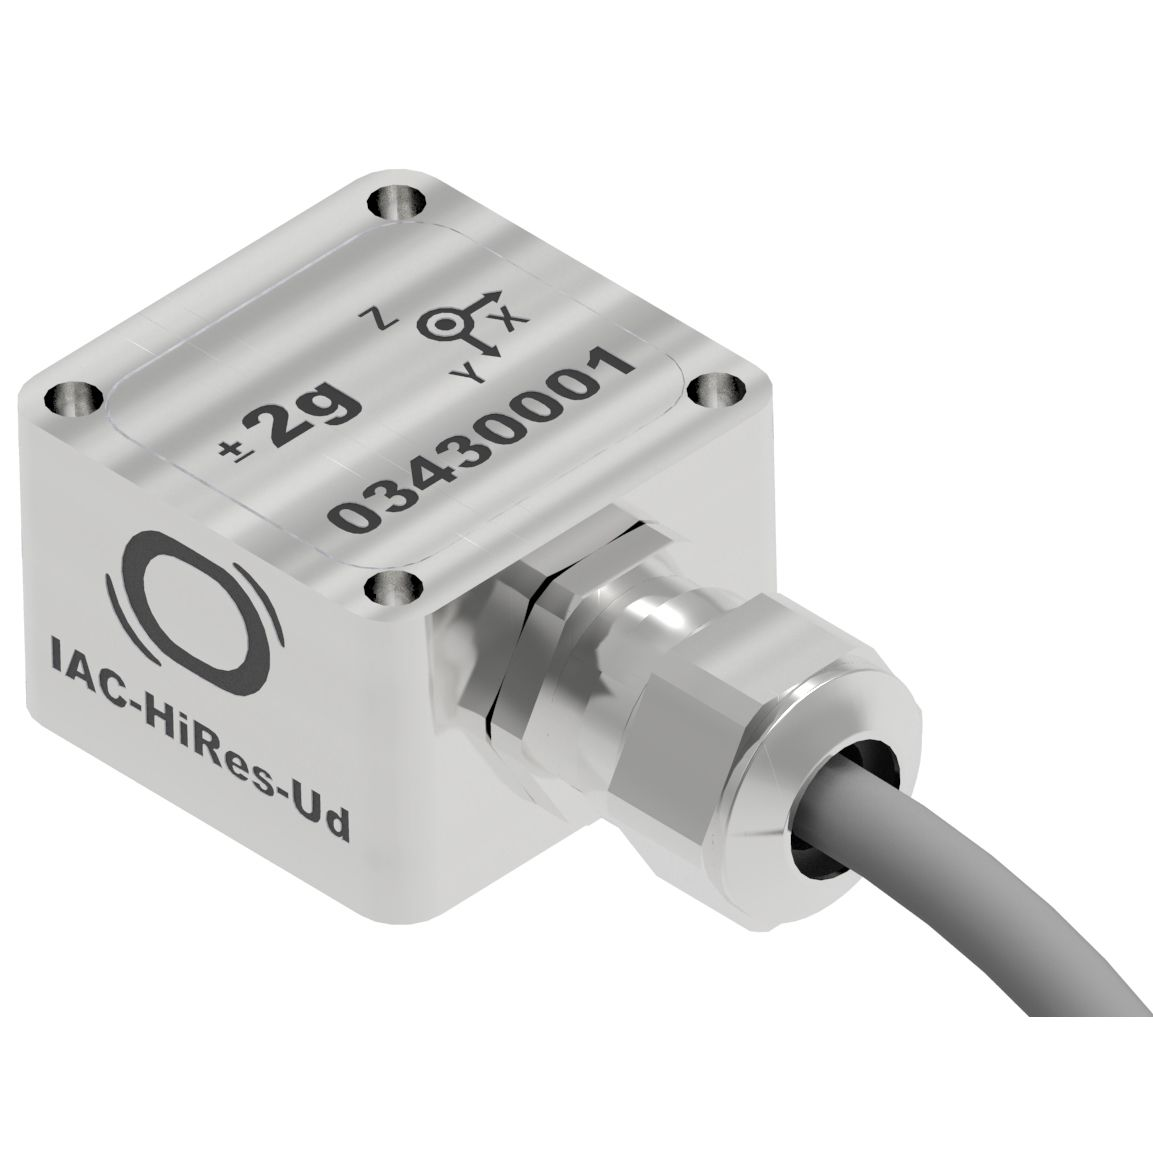
\includegraphics[height=\linewidth]{stumabo/installation/accelerometer_3_axis.jpg}
        \caption{An industrial ACC3D}
        \label{fig:stumabo_acc3d}
    \end{subfigure}
    \caption{Station 1 \textcolor{blue}{blue}: sensor setup}
    \label{fig:stu_station1_b}
\end{figure}
One 3-dimension accelerometer, called \textit{ACC3D} in Figure \ref{fig:stumabo_acc3d}, and a ``mobile cabinet'' was provided to Stumabo, 
which they placed on each of the four machine and roughly kept track of the different positions and operations in a log file.
Unfortunately, this is the only operational data available, with the following structure (see Table \ref{tab:stu_logfile}).
As it can be  seen, despite being in Flemish, it has several tags but with one big issue: start and end time are approximate and do not reflect the data trends collected by the above-mentioned sensor.
% More on that later on. \todo{EB: ``More on that later on.'' troppo informale. E forse anche grammaticalmente sbagliata}

\begin{table}[h]
    \centering
    \begin{tabularx}{\textwidth}{llllll}
        \toprule
        Datum & Start tijd & Stop tijd & Actie & Opmerkingen & Opstelling \\\midrule
        \textit{Date} & \textit{Start time} & \textit{Stop time} & \textit{Action} & \textit{Notes} & \textit{Setup} \\\midrule
        08/10/2021 & 13:19 & 13:29 & Test & Enkel \dots & grote \dots \\ % de slijpstenen van station 1 (grote snede blauwe zijde) draaien. & grote snede blauw  \\ 
        \midrule
        \dots & \dots & \dots & \dots & \dots & \dots \\\midrule
        30/11/2021 & 12:35 & 14:07 & Prod & \dots & \dots \\\bottomrule
    \end{tabularx}
    \caption{Log file structure}
    \label{tab:stu_logfile}
\end{table}

\paragraph{Installation} We must therefore clarify, before we go any further, the industrial setup: in our aid, come the engineering schematics showed in figure \ref{fig:engineering_files};
it consists in three subfigures: the first one (\subref{fig:top_view_line}) represents the same production line we saw earlier at \ref{fig:line_overview}, just from another prospective. 
This view from above makes it easier for us to identify some important elements, e.g.\ how many stones are present for each station.
It is essential to clarify a simple convention: within Stumabo the right side of the line is referred to as \textcolor{red}{red}, \textit{rood} in Flemish, and, in the same way, 
the left side will be referred to as \textcolor{blue}{blue}, \textit{blauw}. 
Speaking about colors, we can now make a direct connection with Figure (\subref{fig:blade_evolution}), which shows us the evolution of the blade during the process.
% Considering that grinding stones turn around their axe sharpening the steel blade.
First it is sharpened, from the 1st \textcolor{blue}{blue} station, on the left side, and then it passes to the 1st \textcolor{red}{red} station, where it will be rolled on the right side. 
Same goes for 2nd and 3rd station, that have two grinders aligned. 

Now that we are aware of how the industrial process works, let's move on to diagram (\subref{fig:local_to_global}).
It represents in more detail how the sensor has been installed and what consequences it has with respect to the coordinate system, 
a somewhat complex issue that has caused several doubts and discussions in the analysis phase. This would therefore appear to be a good point to take stock of the situation.
The accelerometer was installed within the line, adjacent to the stones and close to the blade, by means of a round magnet, as shown in Figure \ref{fig:s1b_foto}.
Moreover, the same device was placed, at different times in different stations, mirrored on both sides, except the last one, for a total of five different locations: 
${S_{1}\textcolor{red}{R}\&\textcolor{blue}{B}, S_{2}\textcolor{red}{R}\&\textcolor{blue}{B}, S_{3}\textcolor{blue}{B}}$ as shown in the bottom part of Figure \ref{fig:top_view_line}.

It follows that \textbf{two} different \textbf{reference systems} are present:
\begin{itemize}\label{item:double_system}
    \item local $(x,y,z)$ for each sensor placement;
    \item global $(X,Y,Z)$ for the entire production line.
\end{itemize}
We can see some refences of this important aspect in the mentioned figures alongside. % here on the side 
This dual model well abstracts the reality, but does not allow a comparison between the various stations, which instead we would like to carry out to achieve the initial goals.
So it will be necessary to transform everything in global coordinates, taking into account two additional factors:
 \textit{sensor orientation} and 
 \textit{installation angle}. 
\begin{figure}[!htp]
    \begin{subfigure}{\textwidth}
        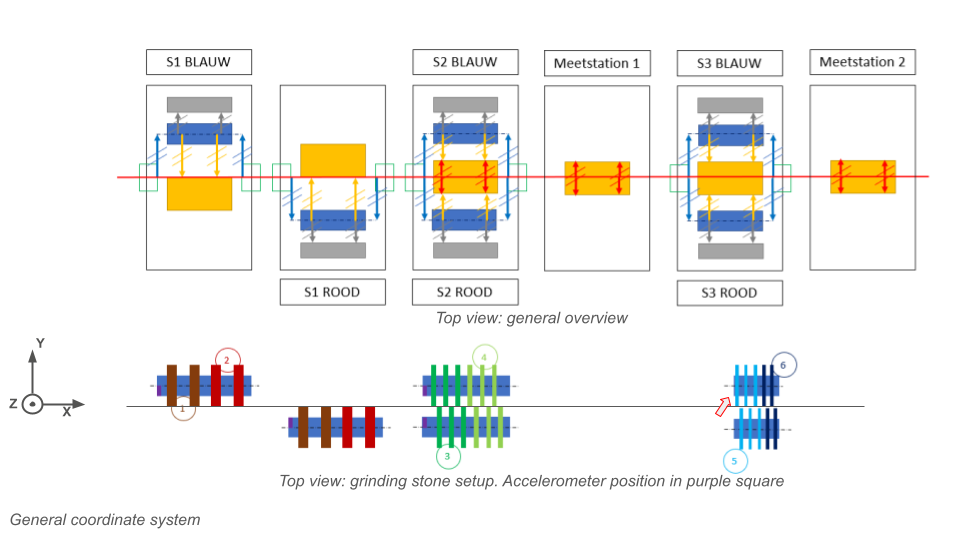
\includegraphics[width=.95\linewidth]{stumabo/installation/general_cordinate_system.png}
        \caption{Top view overview of stations plus grinding stones detail.
            Purple dots on the bottom details are where the $3D$ accelerometer was placed}
        \label{fig:top_view_line}
    \end{subfigure}
    \begin{subfigure}{\textwidth}
        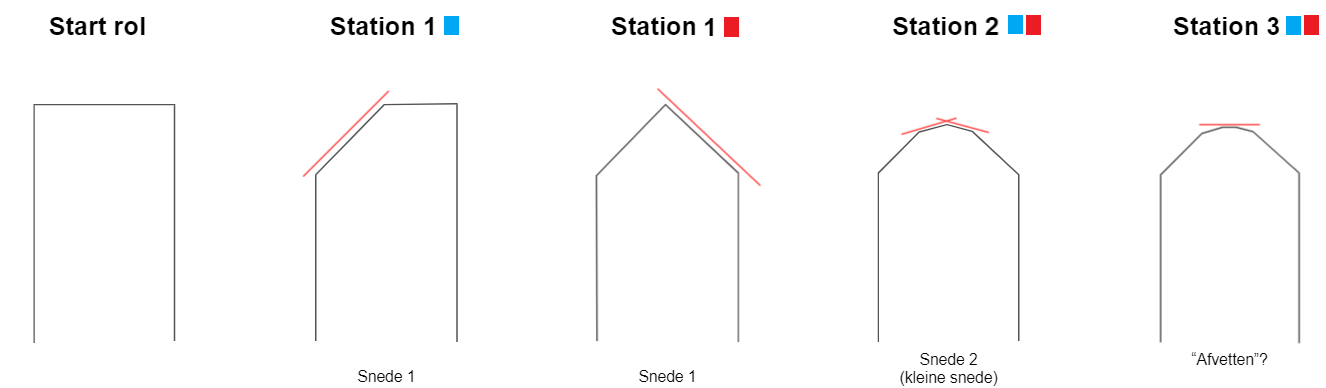
\includegraphics[width=.95\linewidth]{stumabo/installation/blade_processing.png}
        \caption{Blade evolution, a sketched overview of the cut by station}
        \label{fig:blade_evolution}
    \end{subfigure}
    \begin{subfigure}{\textwidth}
        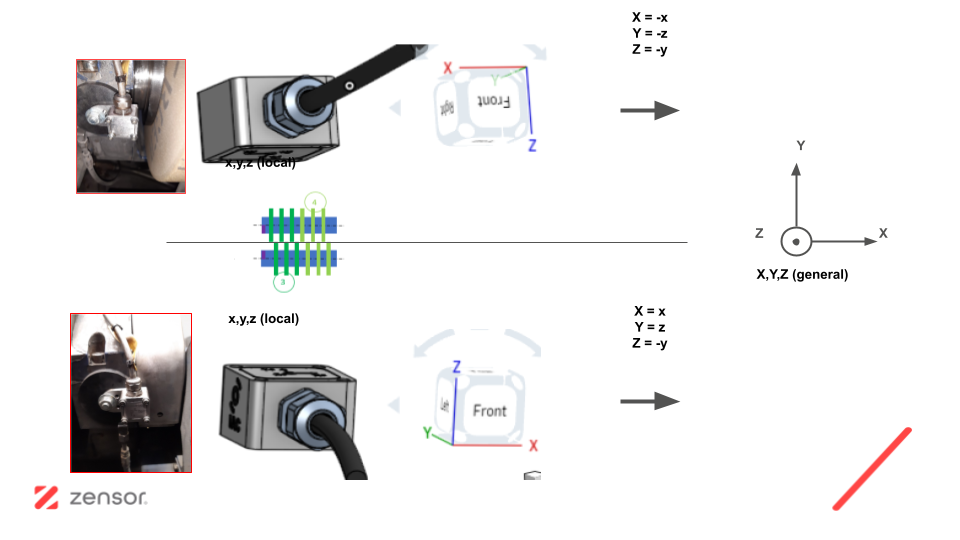
\includegraphics[width=.95\linewidth]{stumabo/installation/local_to_global.png}
        \caption{From local to general coordinate system, top view}
        \label{fig:local_to_global}
    \end{subfigure}
    \caption{Engineering schematic are also important during analysis}
    \label{fig:engineering_files}
\end{figure}

\begin{itemize}
    \item \textbf{Sensor Orientation}: 
    going back on Figure \ref{fig:stu_station1_b}, we can see how the sensor has been installed horizontally, with the $x$-axis as parallel as possible to the blade ($X$) with 
    the help of a level. \todo{EB: check English: ``tolerates''? DG: esiste ed è usato}
    This tolerating some errors due to disturbing factors such as color, dirt and imperfections of the metal.
    Furthermore, the latter is installed upside down, i.e.\ parallel to the $Z$ axis as shown in the Render \ref{fig:s1b_render}.
    \item \textbf{Installation Angle}:
    We had to take also into account that the machines have various angles to the ideal $Z$-axis, this was measured on site and varies from station to station, from 5° to 12° degrees.
\end{itemize}
We will delve into both aspects in the final stage of analysis, but now we would like to clarify following equation-mapping (\ref{eq:op}) from \textit{local} to \textit{global} coordinate.
Here $\widehat{widehat}$ stands for the \textit{rotation} operator and $\underline{underline}$ for \textit{transposition}. 
\begin{equation}
    \left\{ \begin{array}{cl}
        x = \alpha & \Rightarrow  \ x = \widehat{\alpha} \ \Rightarrow  \ X = \underline{\widehat{\alpha}} \\
        y = \beta & \Rightarrow  \ y = \widehat{\beta} \ \Rightarrow  \ Y = \underline{\widehat{\beta}} \\ 
        z = \gamma & \Rightarrow  \ z = \widehat{\gamma} \ \Rightarrow  \ Z = \underline{\widehat{\gamma}}
        \end{array} \right.
    \label{eq:op}
\end{equation}
We now move on to the following phase.

\paragraph{Data Management}
As stated previously a single sensor was placed in different locations, remaining on for the duration of the ad hoc project. We will therefore have a single data stream.
The data flow is as follows: from the sensor to the cabinet to AWS and, finally, InfluxDB.
\begin{figure}[ht]
    % Mettere più grandi?
    \begin{subfigure}{.495\textwidth}
        \includegraphics[width=\textwidth]{stumabo/analysis/60Hz-raw-vibration.pdf}
        \caption{\texttt{60Hz} raw vibration}
        \label{fig:stu_60Hz_raw}
    \end{subfigure}
    \begin{subfigure}{.495\textwidth}
        \includegraphics[width=\textwidth]{stumabo/analysis/1Hz-raw-vibration.pdf}
        \caption{\texttt{1Hz} raw vibration}
        \label{fig:stu_1Hz_raw}
    \end{subfigure}
    \caption{\acl{EDA} on 1° block, station 1 \textcolor{blue}{blue}}
    \label{fig:stu_2_raw_data}
\end{figure}

\todo{EB: mi pare che $x$, $y$, $z$ vengano utilizati a volte minuscoli, altre maiuscoli. C'\`e un motivo? Spiegare motivo, oppure, se non c'\`e uniformare notazione} \\
\todo{DG: il paragrafo precedente (installation) è dedicato principalmente a questa tematica ...}
% \todo{EB: gli Hertz normalmente si abbreviano con ``Hz'' non ``Hz''} 
As a reminder: lowercase stands for local frame of reference, while upper is for global as explained before at \ref{item:double_system}.

I would like to point out that, at cabinet level, two separate binary files are created, where $x$ and $z$ channels are stored together and, instead $y$ channel is kept separated. 
Moreover, for each sensor channel, all vibrations are recorded at \texttt{60Hz}, or 60 points per second, for a total of 180 per second (\ref{sub@fig:stu_60Hz_raw}).
As you can easily imagine when you want to visualize, e.g.\ doing some \ac{EDA} as discussed in subsection \ref{subsubsec:eda}, 
and investigate hours and hours of data these are way too many data points.
This is the reason why Lambda\footnote{AWS Lambda is an event-driven, serverless computing platform \url{https://aws.amazon.com/it/lambda/}}, 
during data ingestion, aggregates the data using the mean function, and reduces the frequency to \texttt{1Hz} (\ref{sub@fig:stu_1Hz_raw}), i.e.\ 
performs a down sampling operation. It then saves both streams in the \ac{tsdb} as separate measurements as shown in Figure \ref{fig:stu_aly_overview}. 
It is an important element that will be useful later in analysis phase.

\begin{figure}[ht]
    \begin{subfigure}{.495\textwidth}
        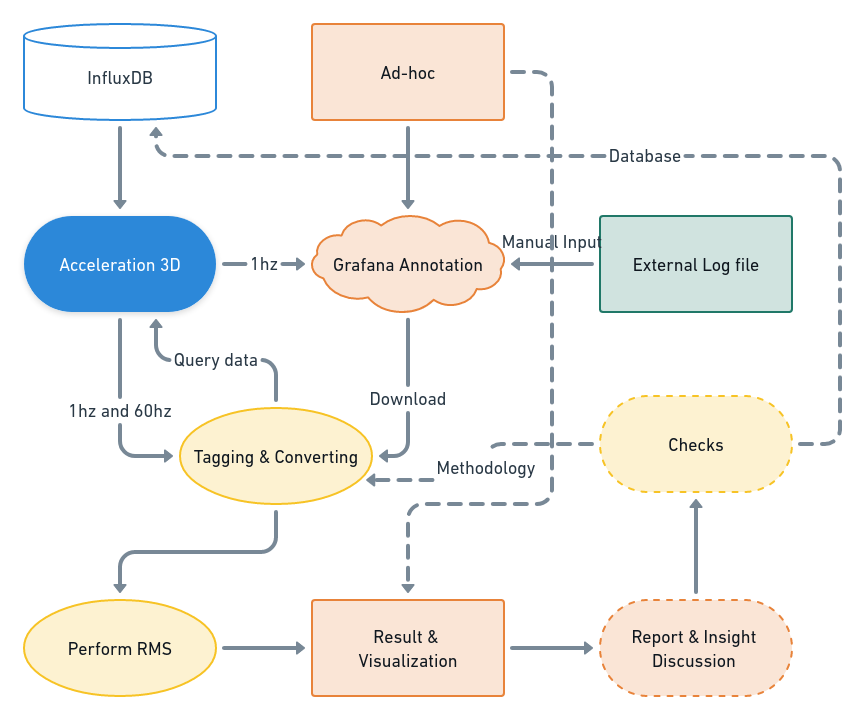
\includegraphics[width=\linewidth]{stumabo/analysis/analysis_flow.png}
        \caption{Data Management and Analysis overview}
        \label{fig:stu_aly_overview}
    \end{subfigure}
    \begin{subfigure}{.495\textwidth}
        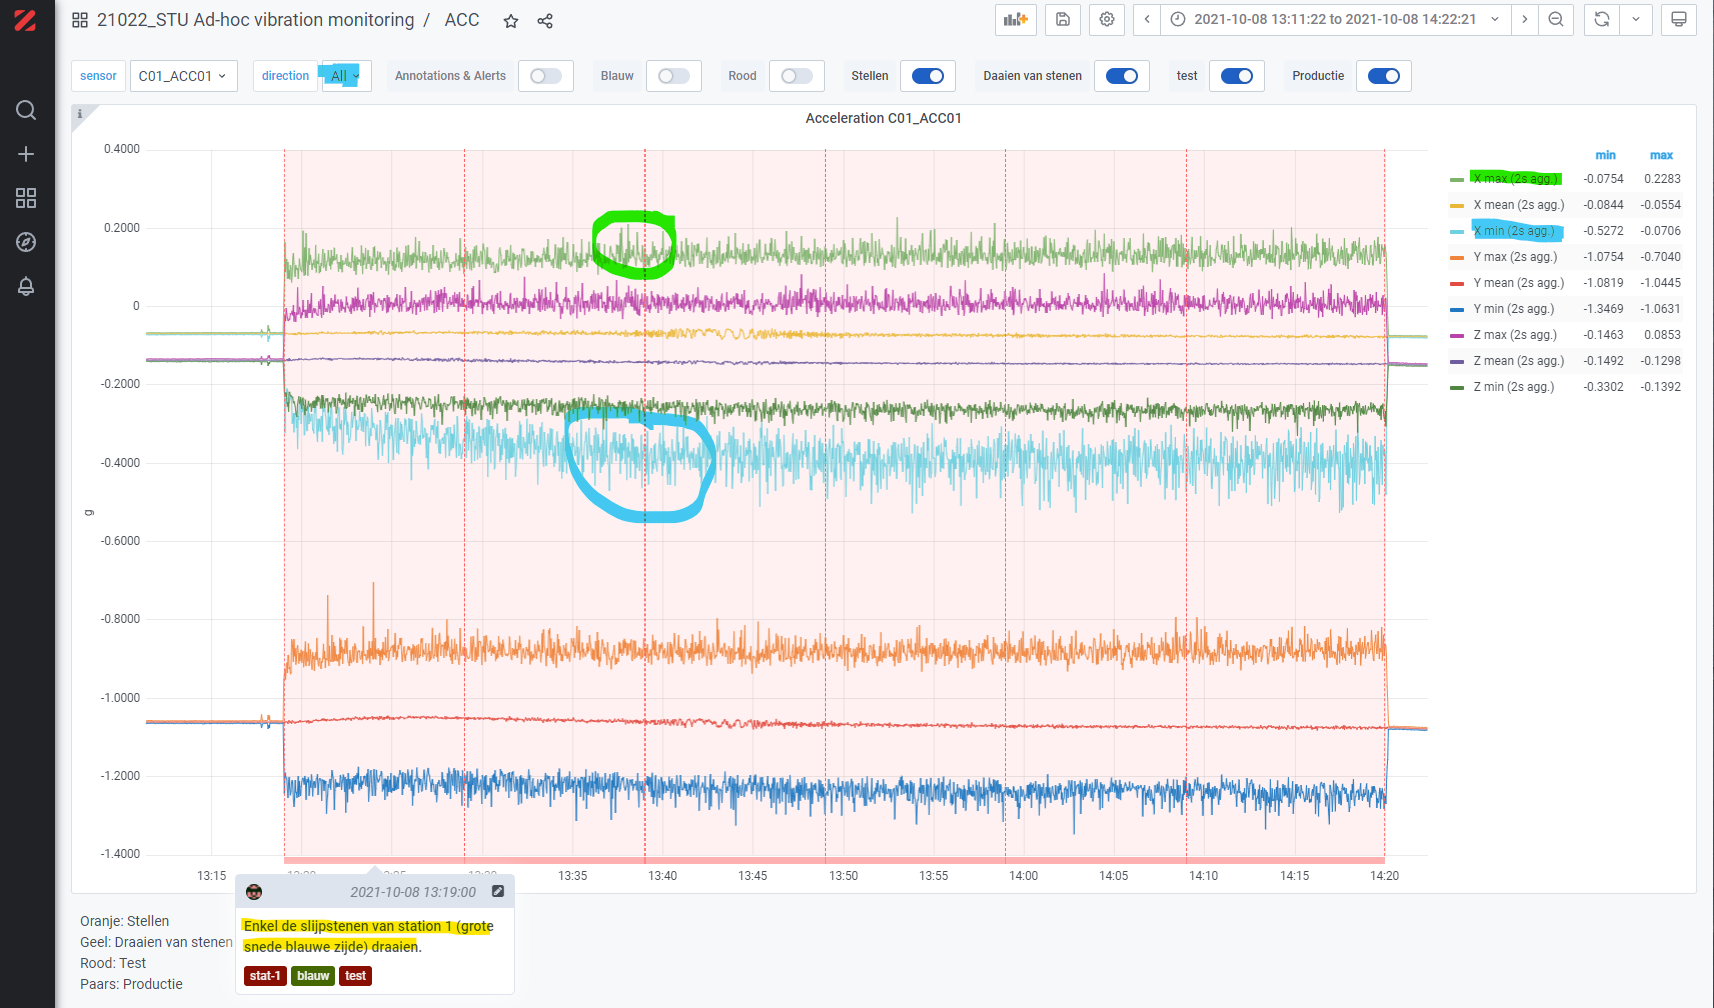
\includegraphics[width=\linewidth, height=4.6cm]{stumabo/analysis/grafana-annotation.png} 
        \caption{Annotation process}
        \label{fig:stu_annotation}
    \end{subfigure}
    % \caption{}
    % \label{fig:stu_2_aly}
\end{figure}

\paragraph{Analysis}
This is where most of my work and time went, my first task was to perform some \acl{EDA} over the \texttt{acc\_1Hz} measurement using Grafana (\ref{sub@fig:stu_aly_overview}).
Since the cabinet was never turned off while sending data for approximately two months, except for five days, between 13/10 and 18/10, it was clear from the start that most of 
the signal was useless, ``flat'' stationary data with no movement e.g.\ during night hours when the servo motors were off. 
Another big problem was that there was no distinction whatsoever between different sensor installation positions.
To solve these and other smaller issues a preliminary data labeling step was performed directly on the visualization tool, using the Excel log file as source of 
operational data, with all the limitations involved. The task was performed in-place using the Annotation UI, dividing the measurement in smaller blocks of variable length 
as demonstrated in Figure \ref{fig:stu_annotation}. While being tedious, it was strictly necessary, otherwise no meaningful analysis could have been performed.

% \todo{EB: troppo informale: Let's go through the procedure together. }
% \todo{DG: non saprei come sostiturlo, quindi rimuovo}

The idea is to isolate relevant data, in other terms data that is available, and we know what it represents keeping in mind we are interested in finding sub zones 
where data seems to be not varying (so much): for instance we would like to exclude the acceleration and deceleration phases of servo motors.
For each client log entry, we create an equivalent annotation entry, with the caveat that there could be more than one behavior block identified per run, so we have two unique identifiers, a Block ID and a Run ID. 
Each block will have several variables like operation \{TEST, PROD, \dots \}, color \{\textcolor{blue}{Blue} and \textcolor{red}{Red}\}, station $\{1,2,3\}$, and so on. 
These variables will be our tags columns $\{n+1, n+2, n+3, \dots\, k\}$ in our final result Table C. To give an approximate order of magnitude, about 110 annotations, hence blocks, were made.
The next step was to download the annotations, using Grafana's REST API, and to transition to a better data structure: from intermediate JSON to structured DataFrame.
Once this metadata was in place, we could proceed with the more complex section of the analytics.
Once again our main concern was to study the amplitude of vibration. So for each \emph{annotated block} we: 
\begin{enumerate}
    \item retrieved ACC data through iterative queries to InfluxDB, using start and end time;
    \item manipulated it, using vector calculus, for performing rotation and translation operations;
    \item returned the \ac{RMS} values for each individual axes $X,Y,Z$;
\end{enumerate}
We are now going to take a closer look at the various operations: % troppo informale? EB: si DG:meglio?
as far as the first one is concerned, nothing too complicated, thanks to zensor library we can easily retrieve our time series data in a shape of a pandas DataFrame.
For the second point, here now we do not dwell too much technical details, it was agreed to combine the two operations into one (see Equation \ref{eq:op}).
So what we end up doing was performing dot product among vector $u$ and matrix $R_X(\phi)$, in formula: $R_X(\phi)u = u$.
With no signs assigned to the angles, that we know from engineering files, the basic translation $+$ rotation matrix on $X$-axis $R_X(\phi)$ is:
\begin{itemize}
    \item \textcolor{blue}{Blue}: \( \left\{ 
        \begin{array}{cl} 
            Y & = \ -y sin(\phi) + z cos(\phi) \\
            Z & = \ -y cos(\phi) - z sin(\phi) 
        \end{array} \right. 
        \Rightarrow  
        \begin{bmatrix}
            1 & 0 & 0 \\
            0 & -sin(\phi) & cos(\phi)  \\
            0 & -cos(\phi) & -sin(\phi)  
        \end{bmatrix} \)
    \item \textcolor{red}{Red}: \( \left\{ 
        \begin{array}{cl}
            Y & = \ y sin(\phi) - z cos(\phi) \\
            Z & = \ -y cos(\phi) + z sin(\phi) 
        \end{array} \right. 
        \Rightarrow
        \begin{bmatrix}
            1 & 0 & 0 \\
            0 & sin(\phi) & -cos(\phi)  \\
            0 & -cos(\phi) & sin(\phi)  
        \end{bmatrix} \)
\end{itemize}
Lastly for the third step is important to point out that, for each direction, before the RMS is calculated, the average of the time-block is determined. 
This average will be subtracted from the array values, as to only monitor the RMS of the relative acceleration.

These three operation were combined in one python function and used alongside Pandas internals. So the methodology was firstly ``called'' on \texttt{1Hz} data for testing the procedure, that took approximately $15$ minutes of CPU time, 
and then on the higher frequency data, \texttt{60Hz} where instead took more than $4$ hours. At Figure \ref{fig:stu_3_rms} we observe three plots.
For all of them we have common elements. The x-axis label is our block identifier (Block ID), while on the y-axis represent the overall RMS value of the block itself. 
It is quite evident how the two graphs represent similar signals but of different order of magnitude. In case \ref{sub@fig:stu_1Hz_rms} we have a $[min, max]$ range of $[0,20] * 10^{-4}$ 
while in \ref{sub@fig:stu_60Hz_rms} is $[0,25] * 10^{-2}$ which makes direct comparison difficult, see Plot \ref{sub@fig:stu_1_vs_60}.
In particular, the \texttt{60Hz} trend seems to be more constant and gradual, while \texttt{1Hz} is characterized by strong peaks. It is clear that station 2 cause most of the vibration, 
as we would expect, by his design with two engines closer to each other.

\begin{figure}[htp]
    \begin{subfigure}{.495\textwidth}
        \includegraphics[width=\textwidth]{stumabo/analysis/1Hz-ad-hoc.pdf}
        \caption{\texttt{1Hz} RMS values}
        \label{fig:stu_1Hz_rms}
    \end{subfigure}
    \begin{subfigure}{.495\textwidth}
        \includegraphics[width=\textwidth]{stumabo/analysis/60Hz-ad-hoc.pdf}
        \caption{\texttt{60Hz} RMS values}
        \label{fig:stu_60Hz_rms}
    \end{subfigure}
    \begin{subfigure}{\textwidth}
        \includegraphics[width=\textwidth]{stumabo/analysis/1Hz-vs-60Hz.pdf}
        \caption{\texttt{1Hz} and \texttt{60Hz} RMS values}
        \label{fig:stu_1_vs_60}
    \end{subfigure}
    \caption{RMS amplitude comparison between low and high frequency data}
    \label{fig:stu_3_rms}
\end{figure}

After all of these operations, we combined \texttt{1Hz} numerical values to the previously prepared metadata to achieve an interesting intermediate result that has approximately this aspect. 
% \todo{EB: ``intermediate'' ==> ``intermediate''?}
Run ID and Block ID were removed here for relevance purposes (see Table \ref{tab:stu_intermediate_res}).  
These results were then discussed and checked with a more experienced colleague, who had more domain knowledge. 
He also continued with the analysis, comparing, for example, different stations for the same type of operation. 
I decided not to discuss his insights, here in this report, as they are not the result of my work but a more direct consequence.
% TEST    = Test   
% DASTE   = Draaien van stenen   
% STEL    = Stellen   
% PROD    = Productie 
\begin{table}[ht]
    \centering
    \begin{tabularx}{\textwidth}{@{}lllllllll@{}}
    \toprule
    start & einde & actie & kant & stat & draaien & $X$ & $Y$ & $Z$ \\ \midrule
    13:19:01 & 13:29:01 & TEST & \textcolor{blue}{B} & 1 & 1 & 131 & 176 & 592 \\ 
    13:29:01 & 13:39:00 & TEST & \textcolor{blue}{B} & 1 & 1,2 & 160 & 143 & 461 \\  
    13:38:58 & 13:49:01 & TEST & \textcolor{blue}{B} & 1 & 1,2,3\textcolor{blue}{B} & 132 & 166 & 356 \\ 
    13:48:59 & 13:59:00 & TEST & \textcolor{blue}{B} & 1 & 1,2,3\textcolor{red}{R} & 113 & 149 & 244  \\
    13:59:00 & 14:08:59 & TEST & \textcolor{blue}{B} & 1 & 1,2,3\textcolor{blue}{B},3\textcolor{red}{R} & 145 & 143 & 217 \\ 
    14:09:00 & 14:20:00 & TEST & \textcolor{blue}{B} & 1 & 1,2,3\textcolor{blue}{B},3\textcolor{red}{R},4 & 176 & 153 & 294 \\ 
    \dots \\
    10:04:00 & 12:35:00 & DASTE & \textcolor{blue}{B} & 3 & 1,2,3\textcolor{blue}{B},3\textcolor{red}{R},4 & 630 & 542 & 1489 \\
    \bottomrule
    \end{tabularx}
    \caption{intermediate result: numerical RMS \texttt{1Hz} values are given using engineering notation: $10^{-6}$}
    \label{tab:stu_intermediate_res}
\end{table}

\subsection{Conclusion}
Stumabo ad-hoc analysis showed, overall, insightful findings. For instance station 1 \textcolor{blue}{blue} has higher vibration than it should, 
and it will be further investigated with spectral analysis for better identify the root cause.
There was a less intuitive result though: vibration amplitudes (RMS) in $X$ direction, along the blade going through the grinding stone stations,
seemed more prominent than in $Y$ direction, also horizontal but perpendicular to the blade direction.
Before digging deeper into this, we wanted to check on our side if these axes can't have been switched somewhere.

The machines (motor, stones \dots) and stones turning both causes vibrations. As discussed previously, for keeping temperatures low, cooling fluid is sometimes applied to the stones, 
where it is absorbed. When drying, we noticed higher vibrations as the liquid isn't all over the stone anymore, but going to the outside gradually.
Anyway, the turning would intuitively cause more vibrations perpendicular to their rotating axe ($Y$) and ($Z$), not along their axe ($X$), 
but in the analysis we saw relatively higher vibrations along the blade axe ($X$) than perpendicular to it ($Y$), even though ($Z$), vertically, is still highest. 
After successfully double-checking back-end, Lambda configuration and the \ac{PLC} programming, we couldn't confirm 100\% the cabling connection, but with a small margin of 
error, we can confirm that, indeed, $X$ and $Y$ are \textbf{not} switched. Further analysis will eventually debunk that. 


% Main concern: amplitude of vibration
% Run ID, Block ID {0,1,...,n}: for each client log entry – there could be more than one behaviour BLOCK identified per RUN
% Actie (4 tags)
%         TEST     = Test   
%         DASTE = Draaien van stenen   
%         STEL    = Stellen   
%        PROD     = Productie    
% Kant
% Station {0,1,...,4}
% Color 
% {blauw, rood}
% Coolant {true, false}
% \begin{figure}[ht]
%     \includegraphics[width=\textwidth]{stumabo/analysis/1Hz-vs-60Hz.pdf}
%     \caption{\texttt{1Hz} and \texttt{60Hz} RMS values}
%     \label{fig:stu_1_vs_60}
% \end{figure}
% A potential deeper investigation for the ad-hoc data is being proposed as of February 2022
\clearpage
% it consist of grid-related electricity metrics.
% Other purpose, the fact that they have the 'same' client [although I think they are different research groups], and the differences,
\section{Monitor electricity consumption}
As the section title states, here we propose a possible approach to monitor the energy consumption of a large campus, the \ac{BHC} in Belgium using existing information, that have been collected over several years.
We also outlined some of the practical difficulties encountered in ingesting, analysing, and visualising the data, 
where understanding the underlying context of the project proved to be an important dimension. 
It is therefore relevant to bear in mind that this is a university-oriented project, therefore pragmatic and data-oriented rather than presentation-oriented.
Despite all difficulties, the product is currently up and running, with new data sources on the way.

\subsection{Initial Hypothesis}\label{sub:vub_initial_hp}
\paragraph{Client} 
% with the motto: \textit{"Conquering darkness by science"} 
\ac{GEP} is a joint project of the \ac{VUB} (Free University of Brussels), dutch and English-speaking research university, and the \ac{UZB} (University Hospital of Brussels), 
whose purpose is to develop and operate a research campus in the Research Park of Zellik with a focus on the following three research domains:
\begin{itemize}
    \item Energy and mobility transition.
    \item Hospital of the future, part of \ac{BHC}.
    \item Smart regions.
\end{itemize}
With this research campus, Green Energy Park aims at bridging the gap between research, innovation, realization and exploitation, by acting as a large-scale living lab, expertise and training centre~\cite{Misc:vub_2020_green}.
\paragraph{Context Introduction}
\begin{figure}[ht]
    \fbox{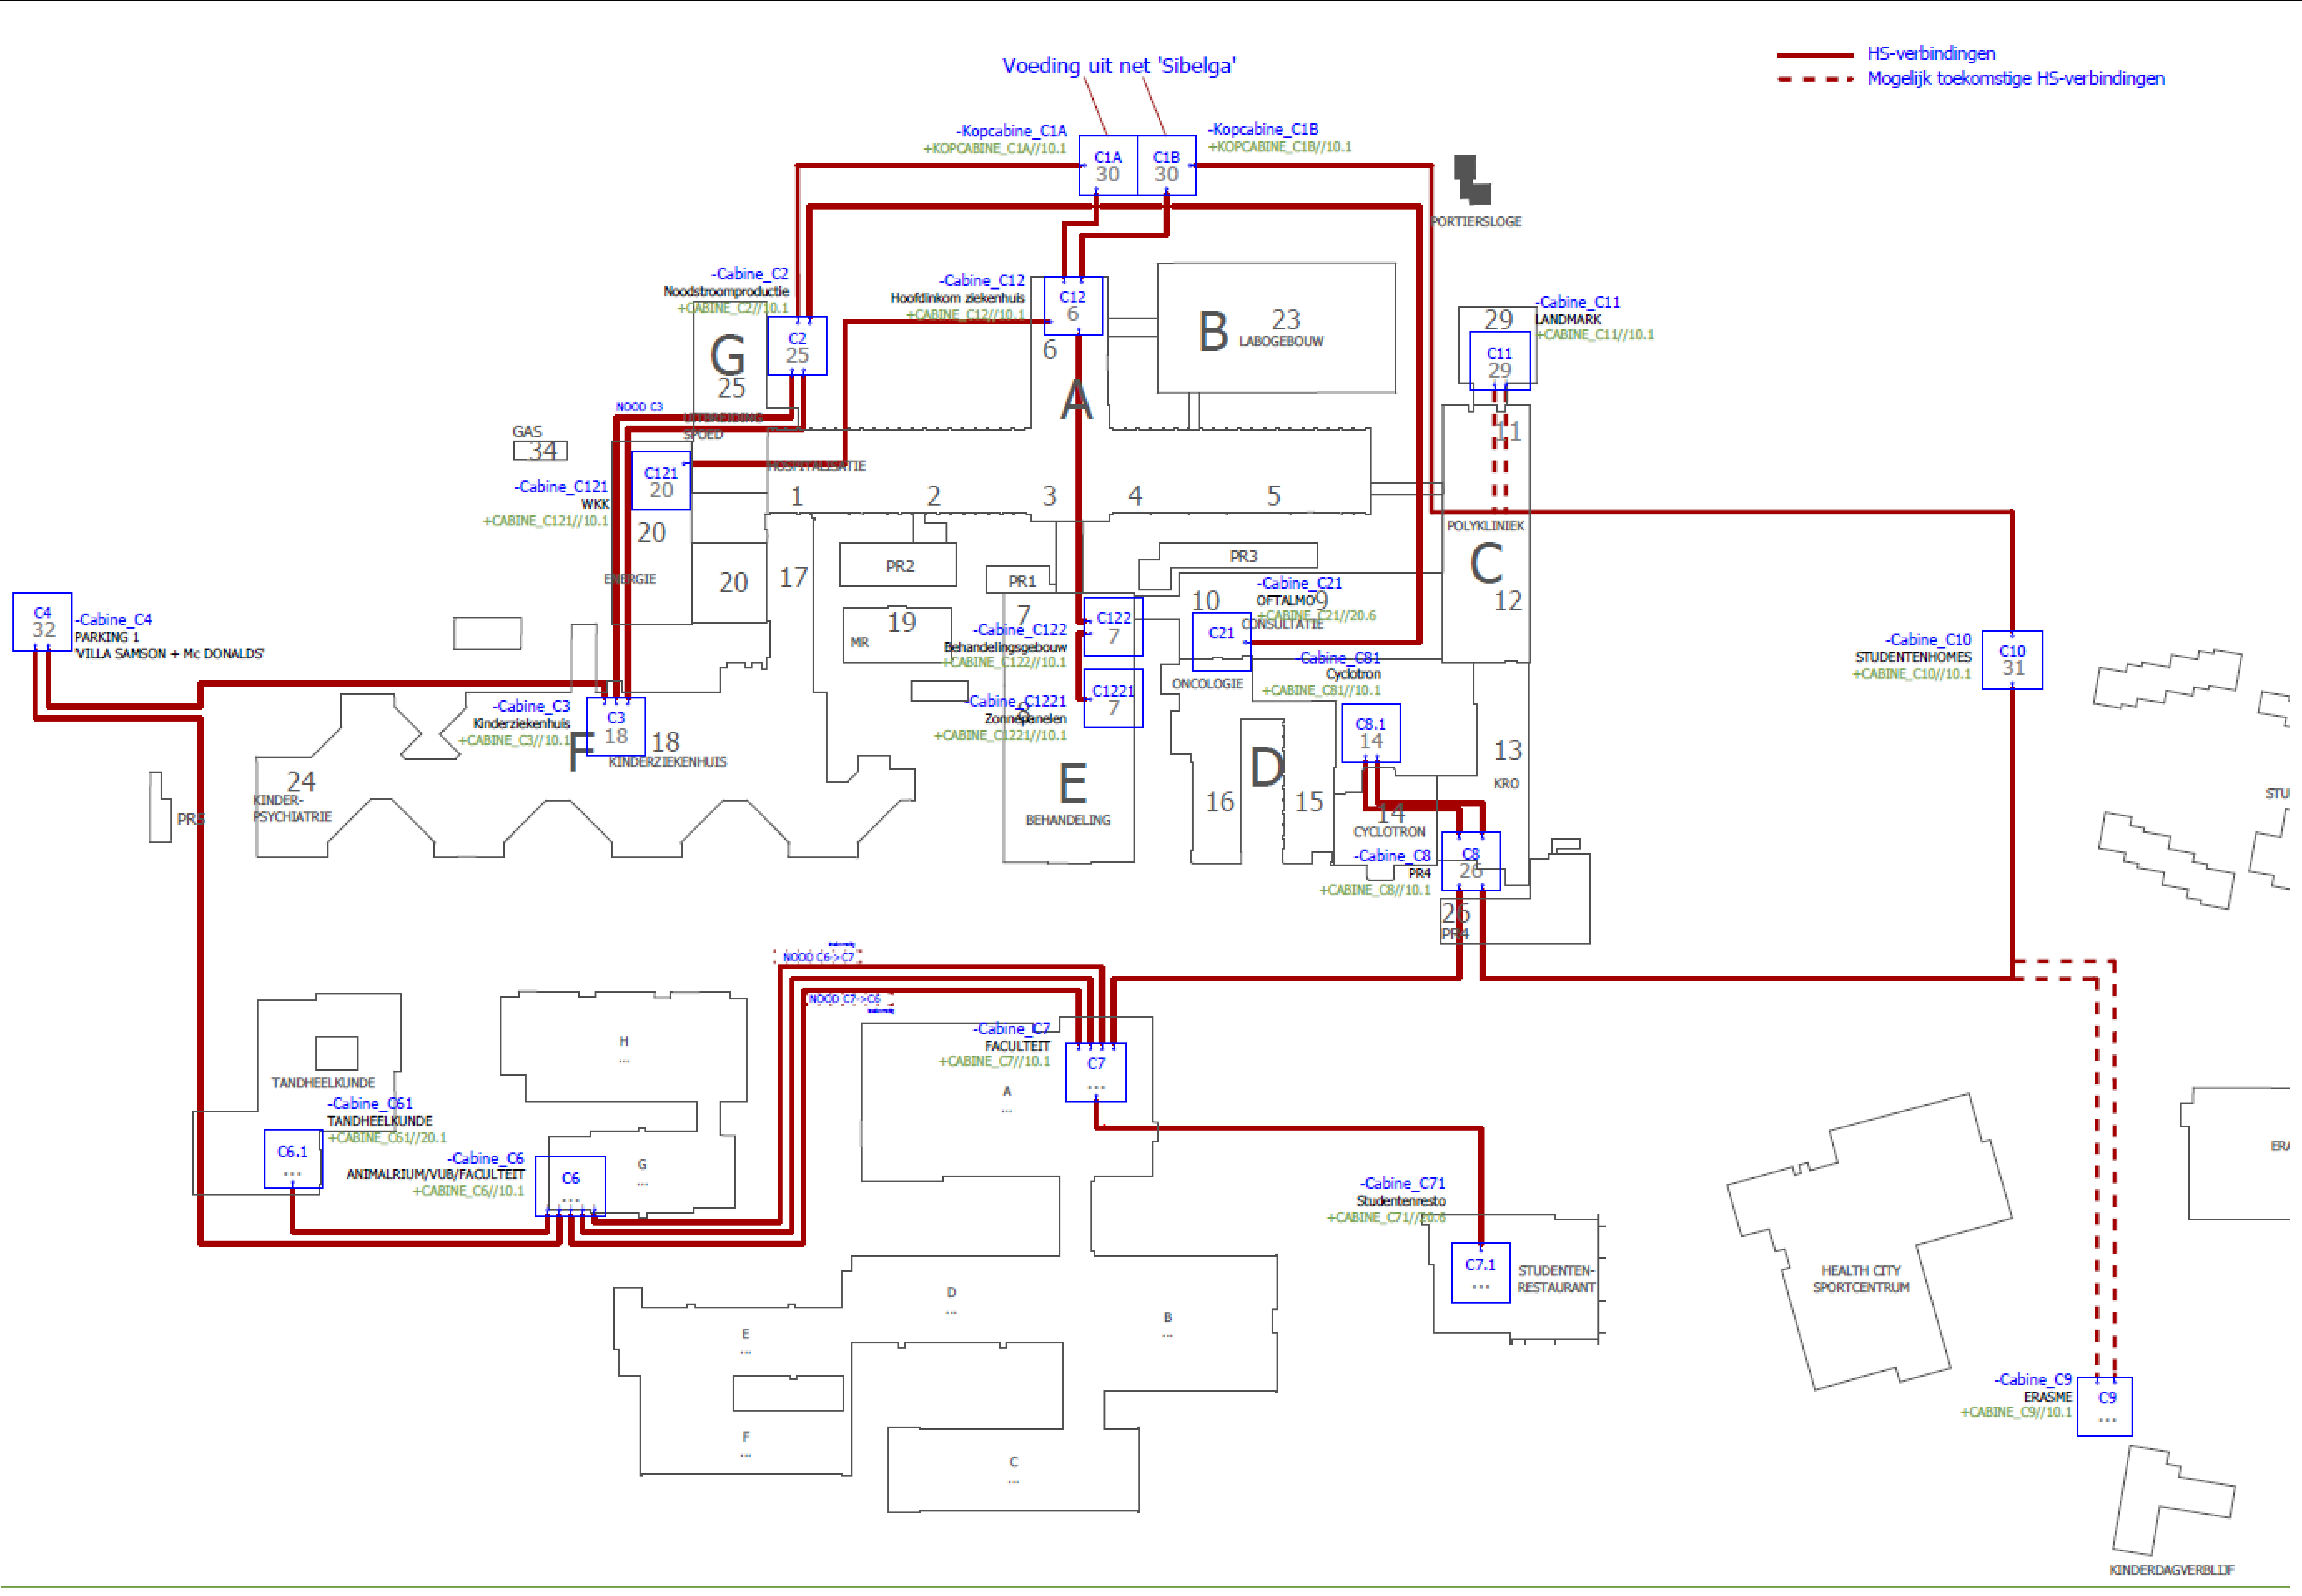
\includegraphics[width=0.97\textwidth]{vub/context/campus_site_layout.pdf}}
    \caption{\acs{UZB} electricity distribution network layout}
    \label{fig:bhc_site_layout}
\end{figure}
As part of this project the \ac{BHC}, containing the academic hospital, is a well-advanced
energy island owning and running a state-of-the-art micro-grid that can work in island mode for five consecutive days.
It includes a thermal and electricity grid, wastewater recovery, a high-speed glass-fibre telecom network and a total of 33 \ac{HV} transformers divided among 18 \ac{HV} substations.
Energy production and storage includes solar PV, \ac{CHP}, three emergency diesel generators,
and a total capacity of 2,5 MWh in battery storage, mainly under the form of UPS.
The micro-grid serves the hospital complex, 250 student dwellings, the faculty of health \& sciences, a primary school and a fitness centre. 
The micro-grid system is conceived to go in island mode with complete automatic transition in maximum 15 seconds in case of critical need and in three minute to comfort need. 
Cutting edge control technology and maximal reliability are the focus points of this demonstration site.

\begin{wrapfigure}{l}{.25\textwidth}
    \centering
    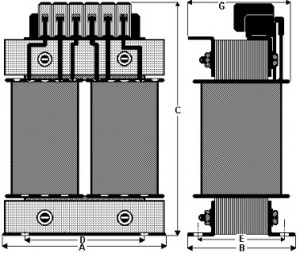
\includegraphics[width=.25\textwidth]{vub/context/trasformatori-uso-sopedaliero-300x253.jpg}
    % \caption{Example of an hospital transformer}
    % \label{fig:transformer_example}
\end{wrapfigure}
The hospital in Jette, our \textbf{main focus}, has its own distribution network, as shown in Figure \ref{fig:bhc_site_layout}.
The network's topology presents a closed-ring shape for increased reliability and is connected to the micro-grid, previously mentioned,  
through two links to nodes C1A and C1B, located at the same place. Each ``node'' of the network is \ac{HV} cabin identified by a code \{C1, C2, \dots, C12\}, with a main transformer.
Furthermore, this cabin can also have connections with one or more ``sub'' transformers, like the one here on the left, 
which are connected to ``consumers'' and/or power sources. The consumers can vary from an individual room to a whole medical department.
% or substations

\subsection{Goal(s), purpose \& critical factors}

% \todo{EB: aggiungere frasetta: ``In this section, we illustrate the company's goals'' o qualcosa del genere. Altrimenti non si capisce.}
The project started at end of July 2020, but data was collected since the 2016/17. 
So, knowing that considerable progress had already been made, I still had the pleasure of contributing to the project in its advanced stages, improving and adding extra features.
Let's see what the project's goals are in the long and short term.

\paragraph{Long term}
\begin{itemize}
    \item[$\circledcirc$] To grow Zensor into the main data hub for the Green Energy Park.
    \item[$\circledcirc$] Minimizing the energy losses and overall consumption, leading to a more profitable operation.
    \item[$\circledcirc$] To identify where the exact sources of this cost are and where the best opportunities for improvement lie.
\end{itemize}

\paragraph{Short term}
\begin{itemize}
    \item[$\circledcirc$] Having a view on the data, centralized and well accessible for multiple people in a structured way.
    \item[$\circledcirc$] Monitoring and tracking energy usage in a production site resulting in more than mere energy bill reductions.
    \item[$\circledcirc$] To improve sustainability reducing energy need and peek request. 
\end{itemize}

\subsection{Project description by phases}
\begin{figure}[ht]
    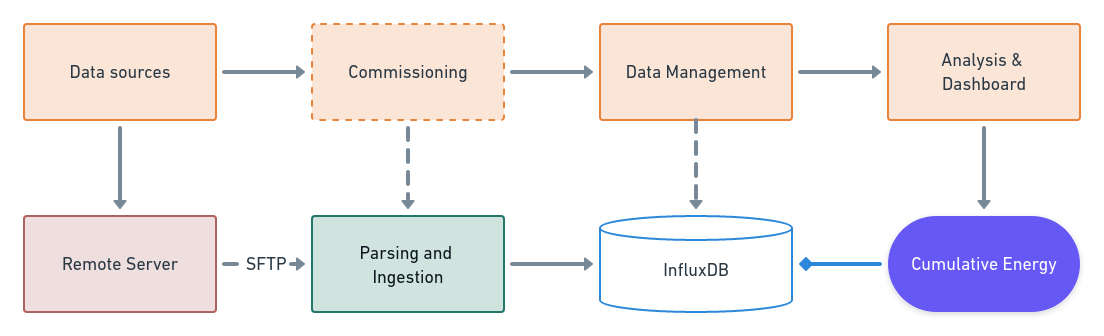
\includegraphics[width=\textwidth]{vub/flowcharts/4_phases.png}
    \caption{\ac{VUB}'s (light) project core stages}
    \label{fig:vub_stages}
\end{figure}
As we have said a few times in the previous section, see Table \ref{tab:phase_diff}, we can have two kinds of projects, full and light. 
This \ac{VUB} project falls into the lightweight class with a ``lighter'' workload, as shown in Figure~\ref{fig:vub_stages}, since the installation and engineering phase are missing. 
Data is provided by the client pre-packaged, saving a considerable amount of time needed for data-collection, but as a downside we have less control over its consistency and quality.
% \todo{EB: non capisco Inglese next ``but there with less control over its consistency and quality'' mi pare manchi un verbo}
On this project, I was primarily involved in the data engineering and analysis aspects, while keeping an eye on the context, introduced earlier, which turned out to be crucial for a successful outcome.

% All the 'items' at that point should also have a link to the manual, spec-sheet... of the component (link to Snipe-It or other database).
\paragraph{Datasources}
MOBI, one of \ac{VUB} research group, has collected through the years several MB of 15-minute data energy-related out of \ac{UZB}'s distribution network.
This limited dataset is currently stored on a remote server in a simple, yet effective way: 
a folder tree, that tries to reflect reality, and it will be our main metadata's source. 

\begin{figure}[ht]
    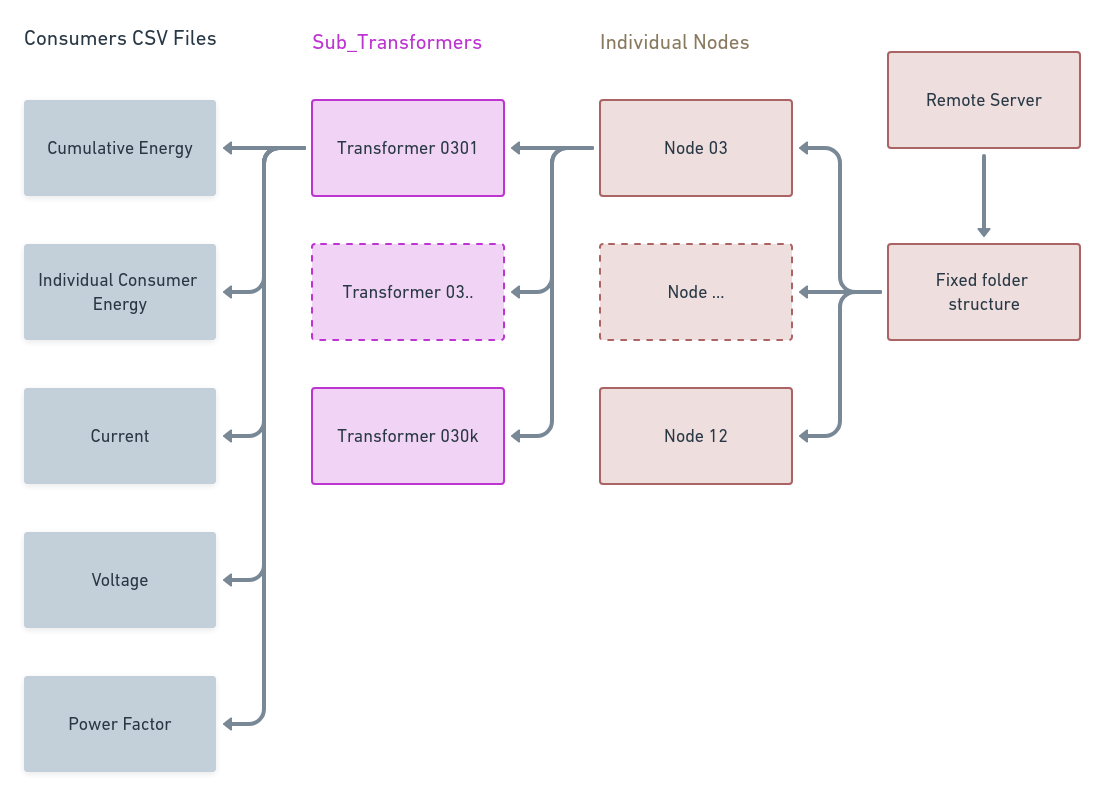
\includegraphics[width=\textwidth]{vub/flowcharts/folder_tree.png}
    \caption{\ac{VUB}'s folder tree structure}
    \label{fig:vub_folder_tree}
\end{figure}
Looking at Figure \ref{fig:vub_folder_tree} from right to left, in a bottom-up manner, should help us clarify the situation. %magari aggiungere colori ai nomi dei diversi livelli come in figura
Starting from the leaves, we found the \texttt{\ac{csv} Files}. Each file shares the same common structure with two columns, \textit{time} and \textit{value}, and multiple rows chronologically sorted.
It can either contain information about a secondary transformer or a consumer/power-source as mentioned before in Section \ref{sub:vub_initial_hp}. 
To make such distinction we must rely on its filename, indicating the hardware source and/or the physical quantity measured.
For example, we could find the file \texttt{Transfo-I3.csv}, referring to transformer's 3° phase current, while file \texttt{Bord LG 03 Radiologie.csv} stores energy consumption of the radiology department.

In our dataset different electricity measurement are present \{current, voltage, power\-factor, energy\}; all taken using the secondary \ac{LV} terminals of the transformers.
How are the different physical quantities organized? 
To answer this question, we go up one level in the tree, moving to the right, stepping up to \texttt{Measurements} where we have five separated directories.
About the energy (kWh): we have to make an important distinction between \textit{individual} or \textit{cumulative}. It can either represent the consumption of one individual consumer or the whole sub transformer, 
ideally it should be the sum of all consumers connected to it.
Instead, for the others (current, voltage e power factor) data is only available at the sub transformer level, not consumer, and in smaller quantities since it was later added to the dataset.

Let's now change the way we traverse the tree, from bottom-up to top down i.e.\ right to left.
From the root (\texttt{Fixed folder structure}), we go down to the \texttt{Individual Nodes} layer, which is self-explanatory. We find in fact a directory for each node of our distribution network, approximately 12. 
This folder contains one or more sub-folder, one for each sub-transformer connected to the same node. Going down even further to the \texttt{Sub transformer} level, same logic applies. Each sub transformer has its own metrics folders.
So that is our connection point with the above argument.
To clarify, let us take the previous example and extend it further: the \texttt{Bord LG 03 Radiologie.csv} will have the following path in a Unix-like OS: \textit{root/NodeC03/Transformer0302/ConsumerEnergy/Bord\dots}.
%So each set of voltage-files is grouped in to a folder

\paragraph{Commissioning \& Data Management}
% Spostare i dati da un server all'altro e digerirli
\begin{figure}[ht]
    \includegraphics[width=\textwidth]{vub/flowcharts/data-management.png}
    \caption{\ac{VUB}'s data ingestion flowchart}
    \label{fig:vub_ingestion}
\end{figure}
Once the university granted us the credentials to remotely access this folder, we could start to manage it by accessing it using \ac{SFTP} over port 9921. % that is periodically
The \textbf{first step} of the ingestion is, as illustrated in the Figure \ref{fig:vub_ingestion}, copying data from \ac{VUB}'s server to Zensor's one. 
This happens periodically as cron job, as mentioned in Section \ref{subsection:script_structure}, also thanks to Python library \texttt{pysftp}. %enumerate?
The script recursively traverses the sftp folder and if it comes across a .csv file, it copies it into the same folder structure as on the server.

Subsequently, for \textbf{step two}, after closing the \ac{SFTP} connection, we can work with our freshly copied data. We traverse, once again, the folder tree, keeping track of
folder names that are going to be important as metadata. Once we are at leaf level, see once again Figure \ref{fig:vub_folder_tree}, we use 
Pandas (\ref{section:pandas}) for handling file reading and inferring the date-time strings format. This switch to a faster parsing method can potentially increase the speed by 5-10x. %parsing
Then we can perform some data cleaning, for eliminating outliers, duplicates and non-numerical values out our DataFrames, one for each file.
Afterwards we tag the respective \textbf{DataFrame} with the necessary information to easily identify it, like description, unit and other metadata previously collected.

Since the files are numerous and of significant size, this series of operations can take a long time. 
Therefore, it was decided to parallelize the whole operation using a pool of processes, not threads. To substantiate this point, here is a small digression: 
in Python, if code is \textit{CPU-bound}, multithreading won't help, because only one thread can hold the Global Interpreter Lock, and therefore run Python code, at a time. 
So, in this specific scenario we need to use processes, not threads, since in multiprocessing, any newly created process will run independently with its own memory space.

Finally, the \textbf{step three} involves writing each DataFrame on the InfluxDB (\ref*{section:influxdb}), our choice for \acl{tsdb}.
This operation, which is already quite optimized, can be easily executed in parallel given the limited concurrency.
As a result, we will have a \textit{``measurement''} for each node, which will contain several series, one for each consumer, easily distinguishable from the others.

% In a second instance they want the entry point to be a map of the campus with the main transformers indicated and with a clickable link on each item such that the data can be consulted. 
\paragraph{Analysis \& Visualization}
\begin{figure}[ht]
    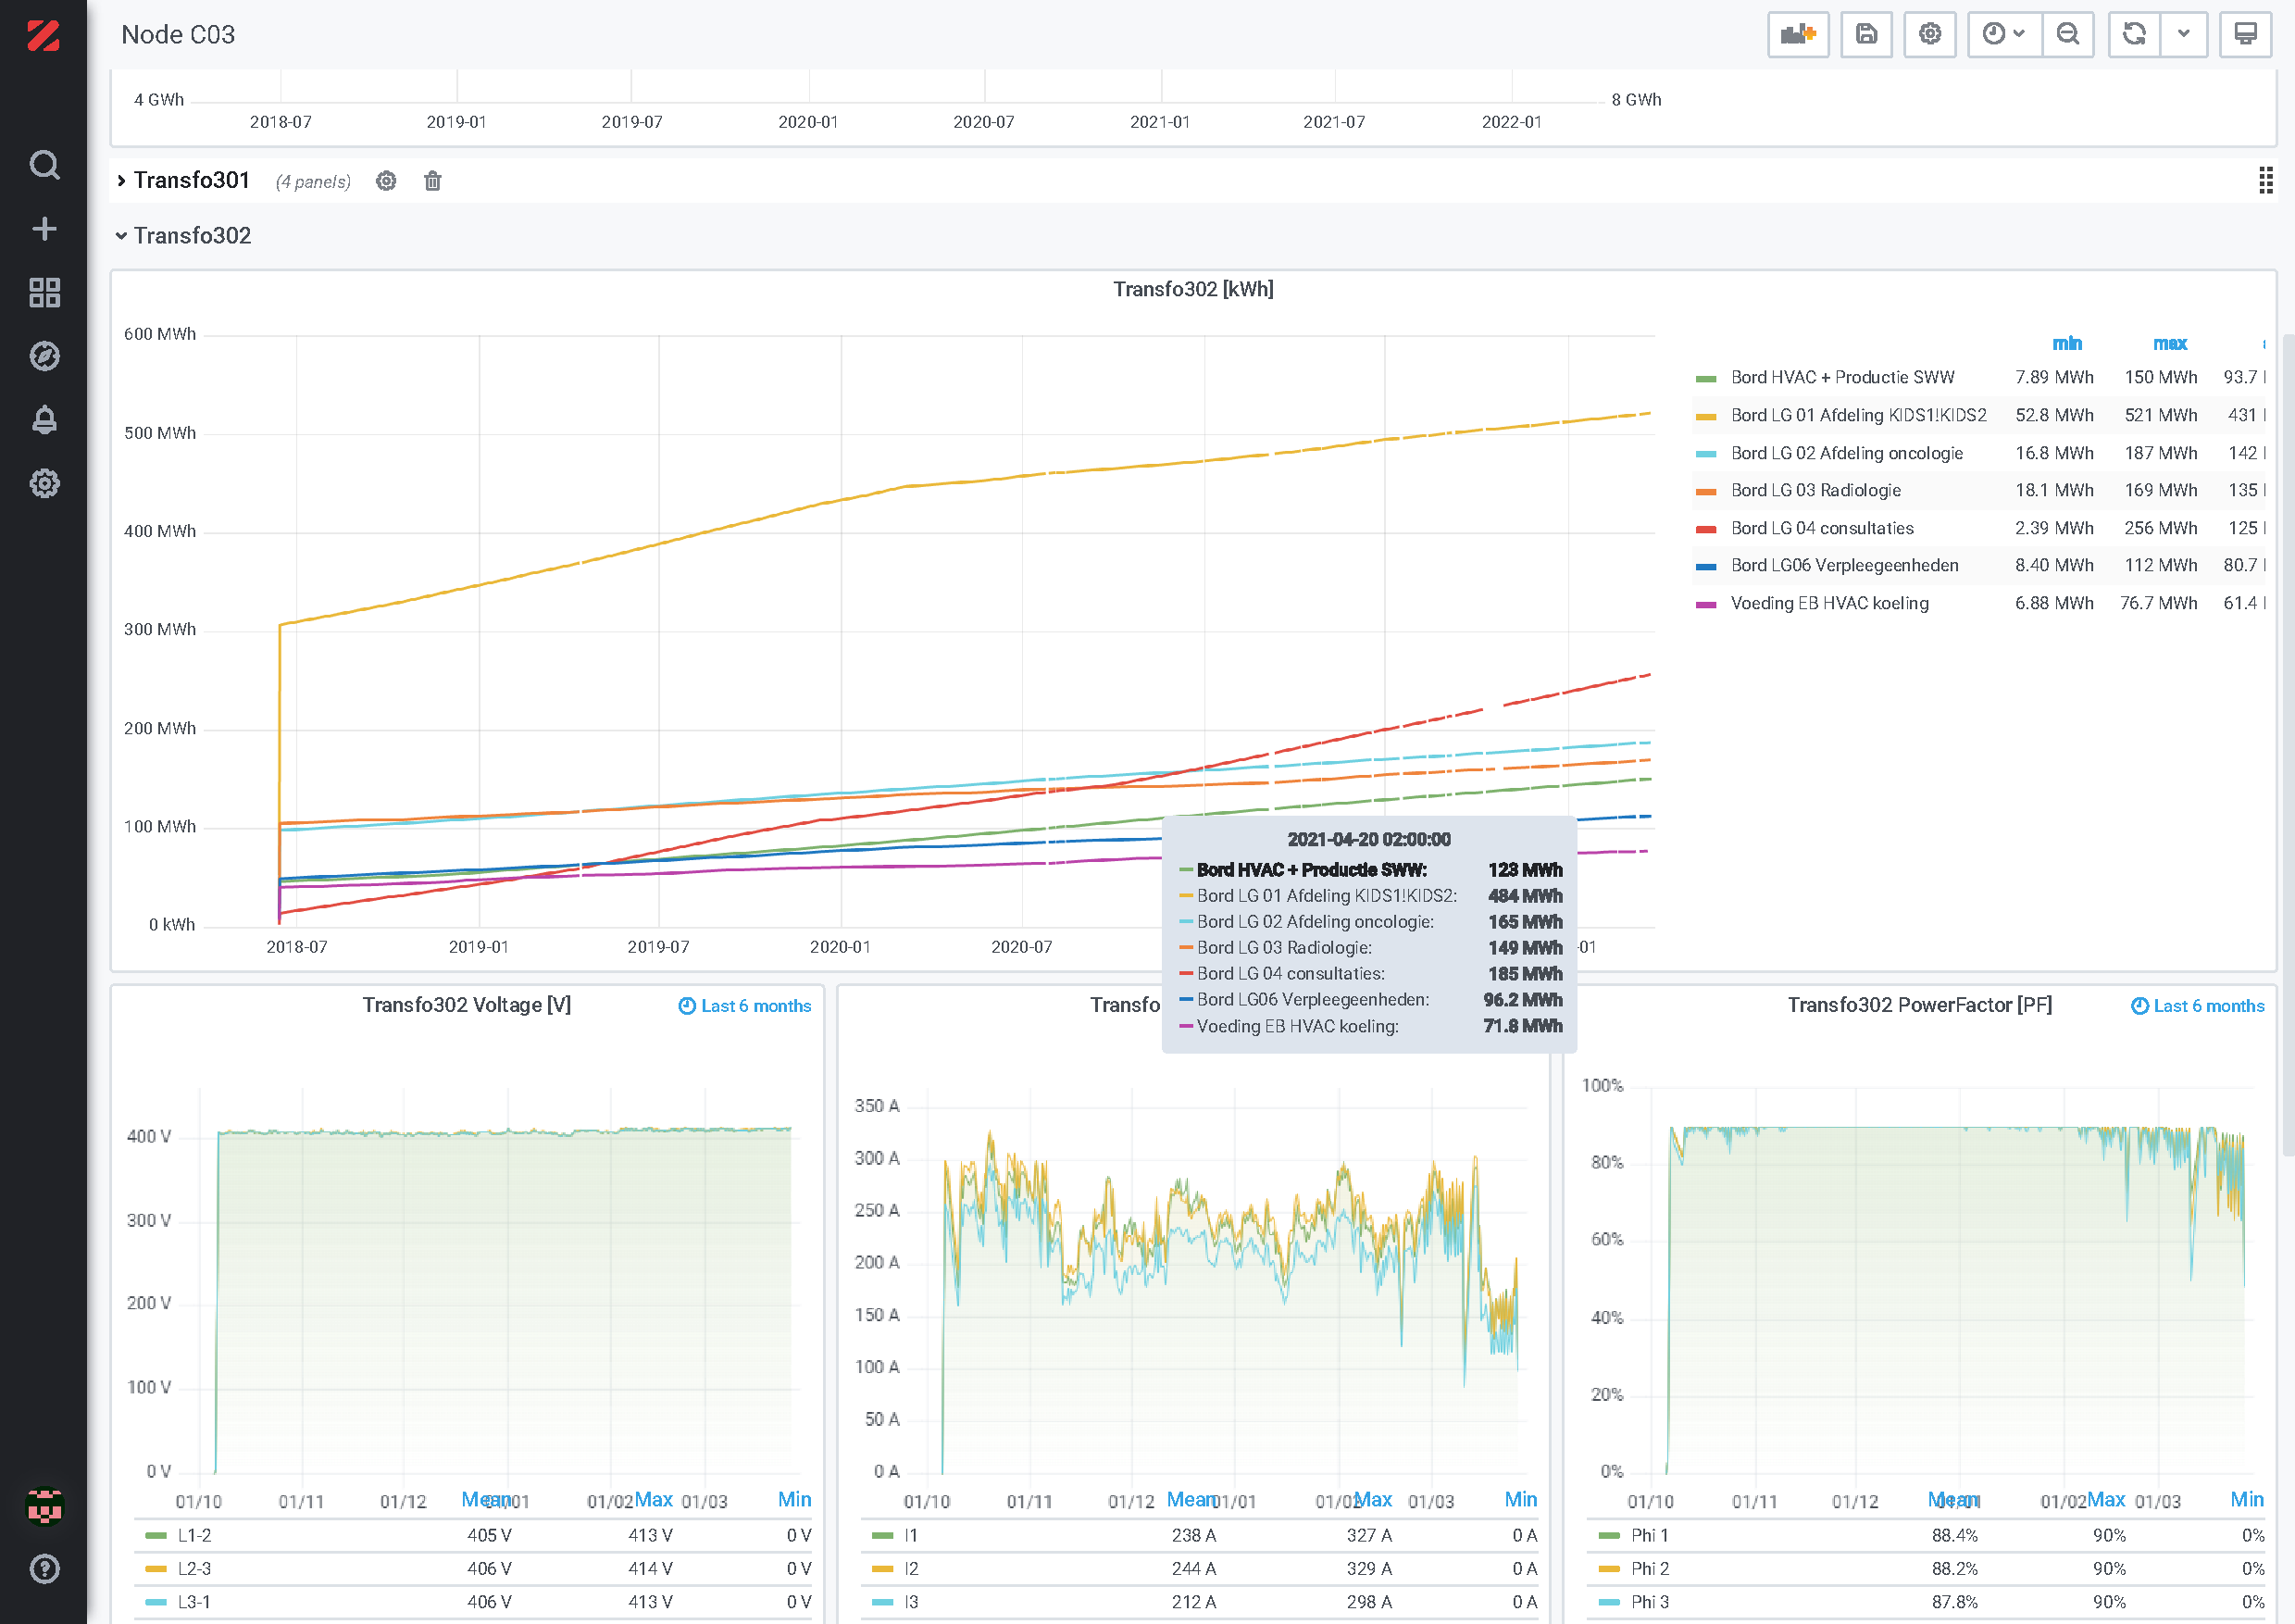
\includegraphics[clip, trim=0 0 0.1cm 3.5cm, width=\textwidth]{vub/grafana/node_c03_transfo302_raw.pdf}
    \caption{Transformer302 raw data dashboard}
    \label{fig:vub_raw_rad}
\end{figure}
To ensure that ingestion has been carried out correctly some basic visualizations is required.
Therefore, we designed the dashboards to share the same structure, same philosophy as the distribution network.
So, each node (\ac{HV} cabin) will have its own page, with a variable number of panels, depending on how many sub-transformers are present. %per node

Taking the Node C3 dashboard as an example, illustrated in Figure \ref{fig:vub_raw_rad}, enhanced with a bit of contextual information: 
the station gives power to the children's hospital, as we can spot references to medical wards in the legend, and has three sub-transformers.
In particular we will focus on the second one and its metrics, where we can recognise some key elements previously discussed.
Starting from the bottom, we find three panels covering transformer's (Transformer 302) voltage, current and power factor, with a minimum six months temporal frame.
As mentioned at the beginning of this segment, these measurements were added at a later stage and are in a smaller volume than the electric energy. 
At this stage of the project, there is not a high interest in performing any analyses on these metrics, besides trend monitoring. 
Directly above, a larger panel visualises the energy consumption of all 7 consumers connected to the transformer.
As we discussed in Section \ref{section:grafana}, \textit{Grafana} allows us to adjust the time window to our liking.
In the time interval chosen, from July 2018 to March 2022, each signal appears to be a monotonously increasing function of time $f(t)$. 
In fact, corresponding data, measured at the \ac{LV} stations, is cumulative: easy to collect and store, but less interesting from an analytical point of view. 
Following this argument, we should not be surprised that, taking a random point (20 April 2021), the different energy consumption values recorded at that instant 
are of a higher order of magnitude [MWh] than expected [KWh].
% We will resume this issue at later stages.

One of the objectives of this project is to provide information on the energy intake of the various nodes, making more effective use of these data. 
The next step is then to calculate appropriate usage statistics, also to answer common questions such as: \textit{what is the average consumption of transformer $x$?}
We now shall examine the workflow of operations necessary for achieving this goal.

\begin{figure}[ht]
    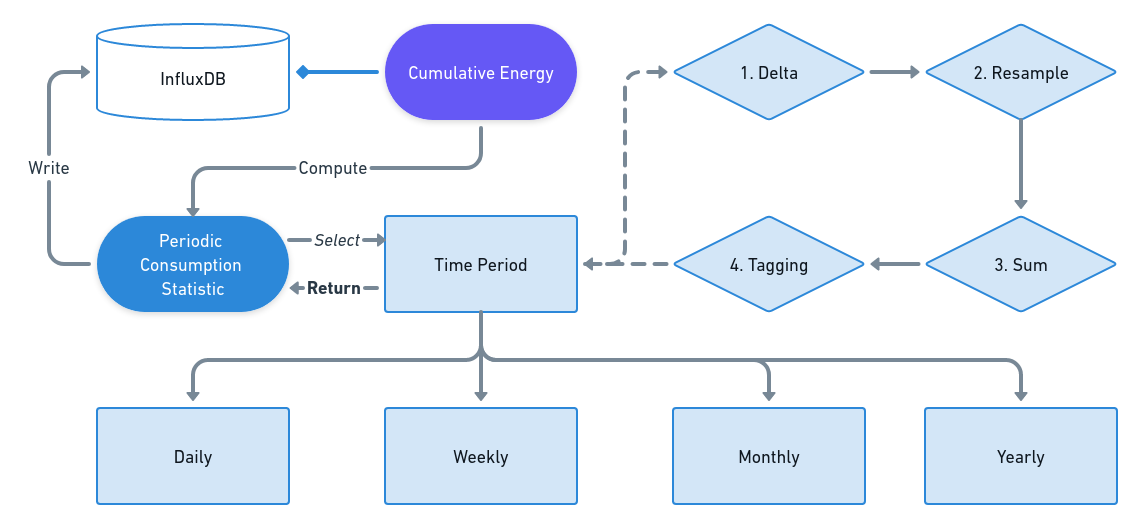
\includegraphics[width=\textwidth]{vub/flowcharts/analystic_flowchart.png}
    \caption{\ac{VUB}'s analytics chart}
    \label{fig:vub_anal_chart}
\end{figure}
Looking at the diagram in Figure \ref{fig:vub_anal_chart}, we can observe that the first necessary step is to choose a time period $T$, daily to yearly.
Ideally, for the end user i.e.\ the VUB researcher, all options will be available, but certainly the daily $T$ is highly informative.
As for the subsequent steps, they are quite intuitive at an abstract level.
\begin{enumerate}
    \item First, following the previous discussion, we calculate how much the series varies. 
    That is, taking two successful points of the signal $x_t$ and $x_{t+1}$ we calculate the delta i.e.\ $\Delta = x_{t+1} - x_t$.
    \item Second, using pandas split-apply-combine approach, as discussed in Figure \ref{fig:pandas_groupby}, we group on our tag columns; then we use the library downsampling 
    functionality for performing a frequency conversion on $\Delta$-data: from 15-minutes to the selected $T$ period.
    \item Third, we compute the group sum, as the apply step and we get our data combined as requested.
    \item Four, we tag the resulting DataFrame with extra information, such as the resulting frequency, quite useful for visualization and querying purposes.
\end{enumerate}

So, all that remains is to visualise the \textit{periodic consumption} statistic in an intelligent way, providing some insights for researchers.
We shall now take a look at two dashboards, illustrated in Figure \ref{fig:vub_2_dashboard}, with several panels using a range of visualisation techniques, but querying the same statistic.
As mentioned in the figure's caption, we are displaying data concerning the preceding case, i.e. the radiology department of the children's hospital.

In detail, starting from dashboard (\subref{fig:vub_stats_v1}), we find, on the top left corner, a panel representing the daily consumption distribution, which is mainly between 20 and 80 kWh. 
On the right side we can see, instead, a pie chart about the proportional average intake per day of the week, where the maximum is Tuesday and the minimum Sunday. 
Finally, at the bottom, we have a status map which gives us, at one glance, a comprehensive view of long-term average daily consumption. 
For instance, we were able to notice that on the \textit{28/12/2022} there was a spike in usage, with a value of 235 kWh.

Turning now to Figure (\subref{fig:vub_stats_v2}), we can see that it consists of three panels. Starting again from the top left-hand corner, 
we have a bar plot, indicating the average energy consumption per day of the week. % averaged over the selected period. 
Note that the y-axis does not start from 0, but from 37.5 to highlight the present differences. 
On the right, we find once again a pie chart, similar representation to that discussed for panel (\subref{fig:vub_stats_v1}).
Finally, at the bottom we see another bar plot, horizontally aligned, visualising the same daily average over a longer period, i.e. a month, with peaks in June and July and lows in October. 
As a minor distinction between the two is that (\subref{fig:vub_stats_v1}) have transparent panels, as contrasting with the white background of (\subref{fig:vub_stats_v2}). 
With these considerations,  we can consider close the discussion, knowing that a few aspects have been left out, to keep the text as relevant and clean as possible.
% \todo{EB: meglio ``we can close the discussion'' o simili?}

\begin{figure}
    \begin{subfigure}{\textwidth}
        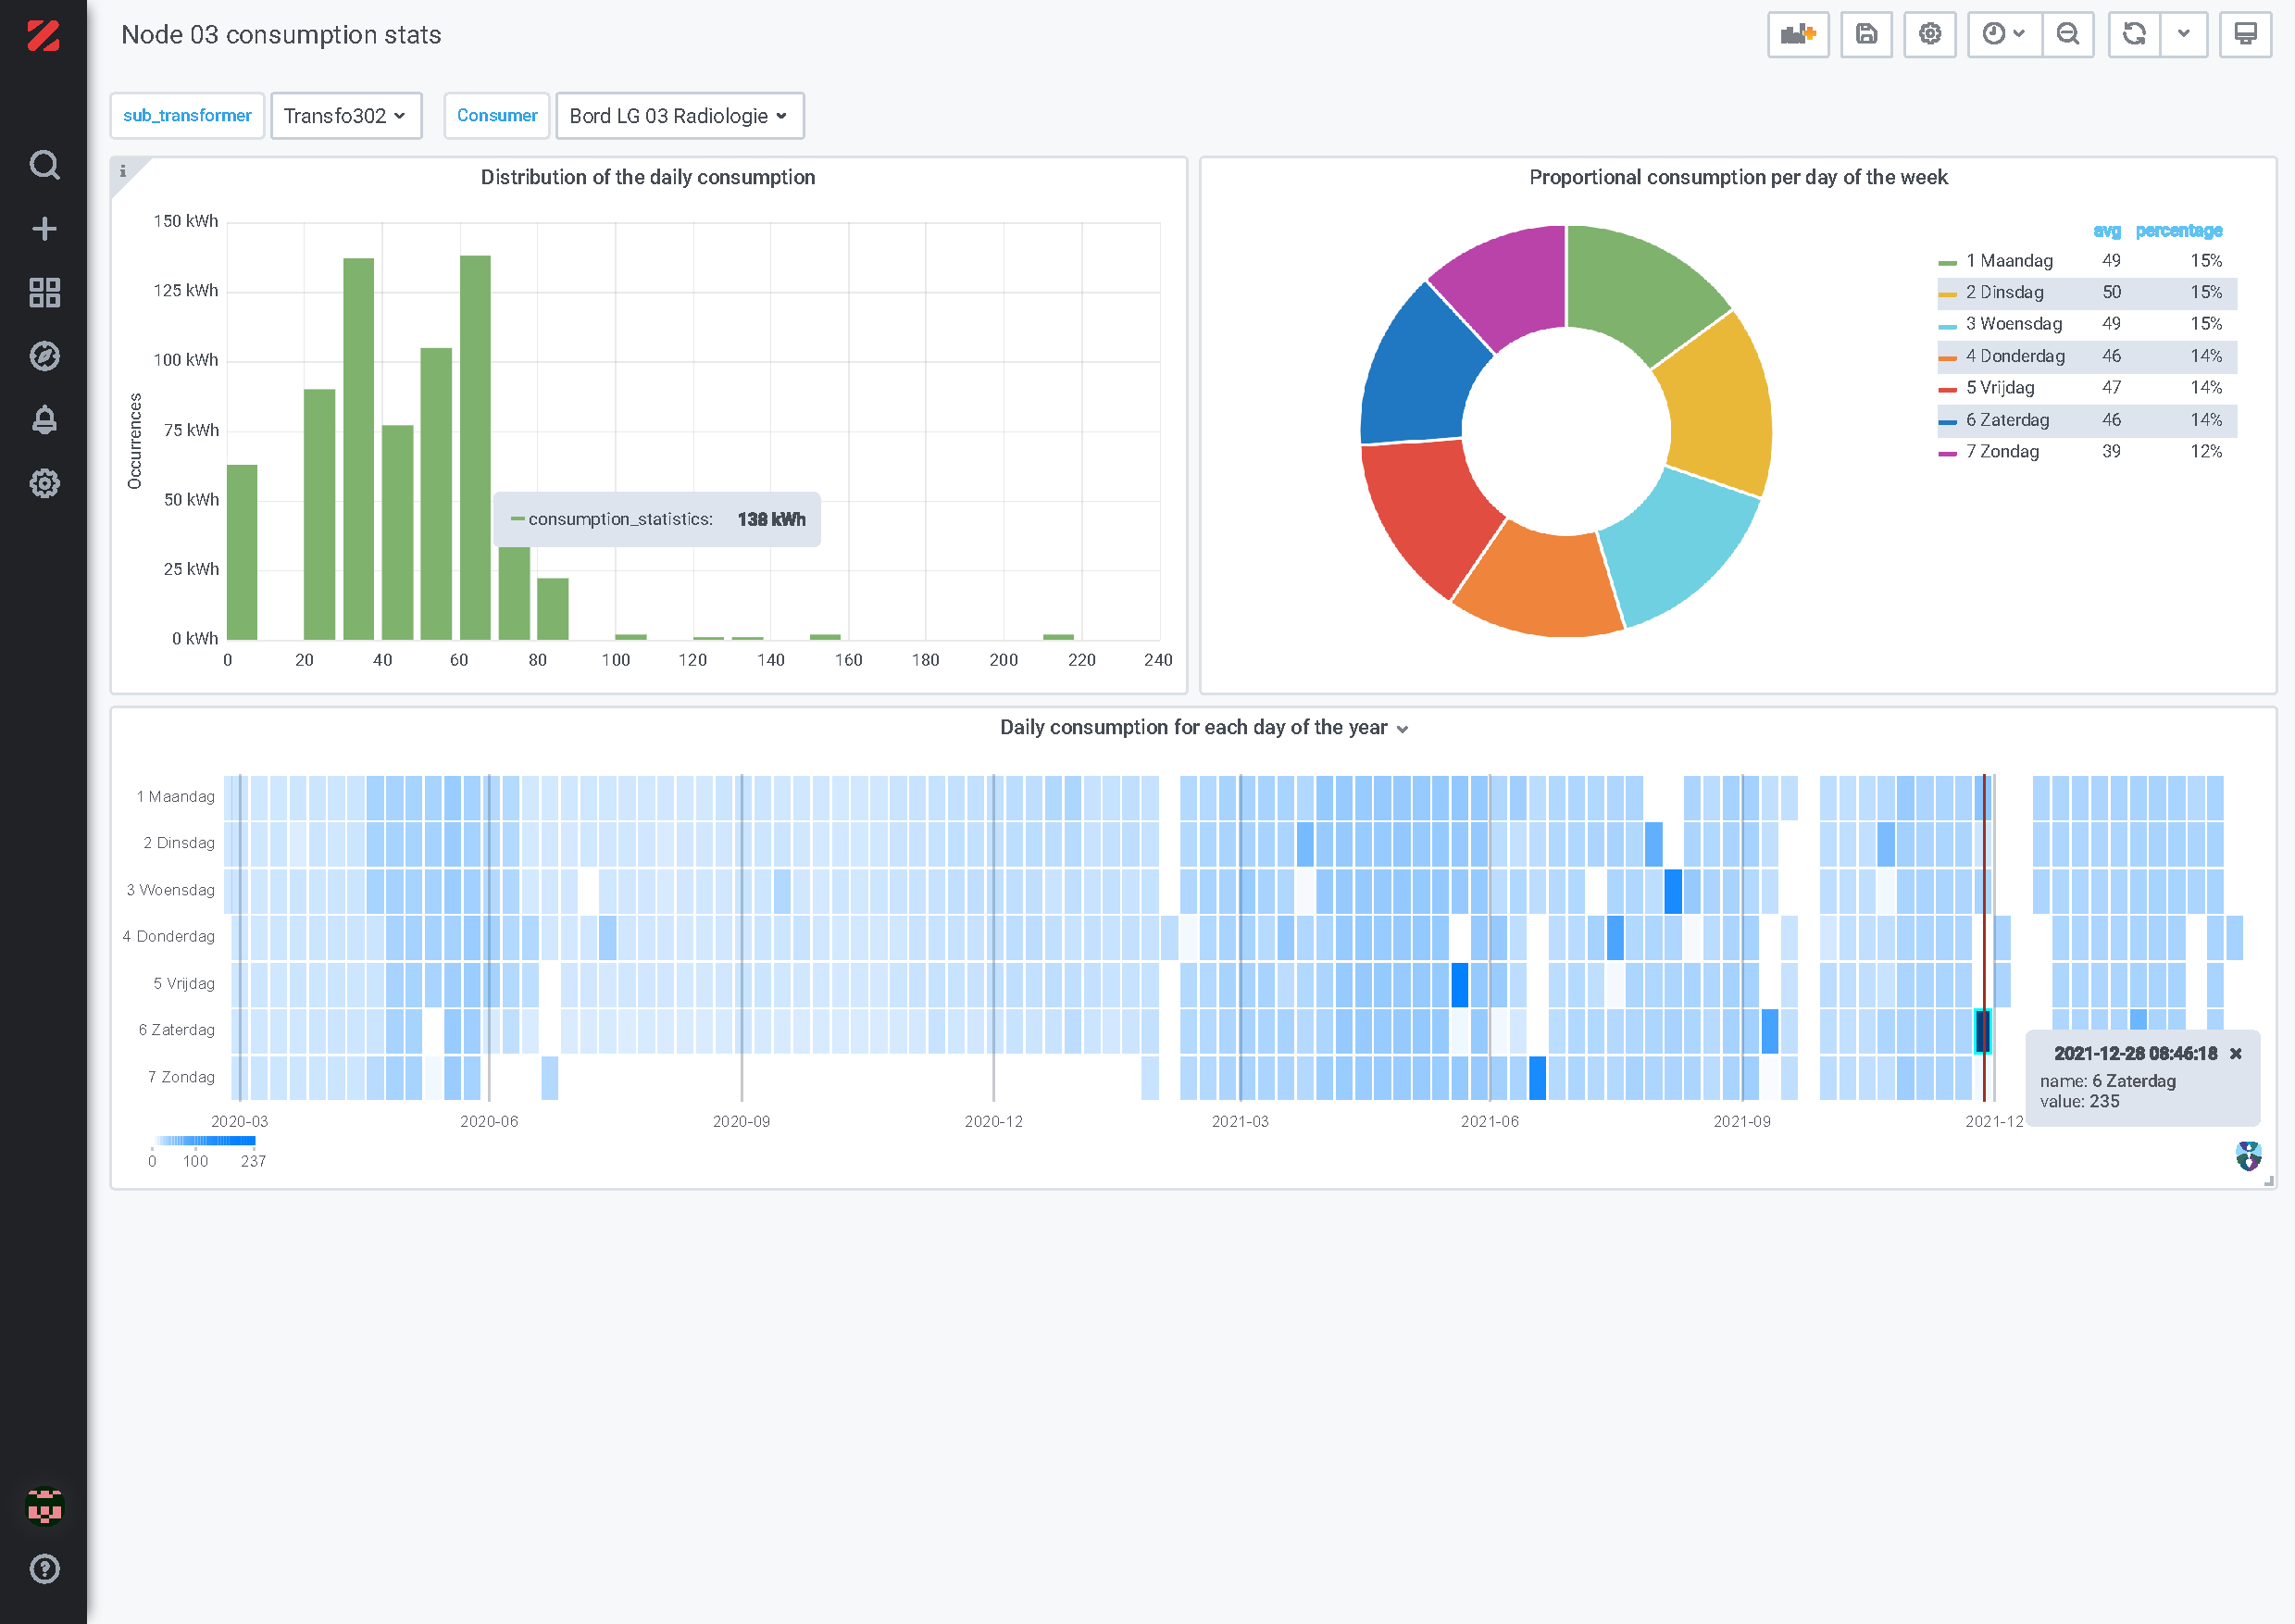
\includegraphics[clip, trim=0 7.5cm 0 0, width=\textwidth]{vub/grafana/node_c03_consumption_stats.pdf}
        \caption{Daily distribution}
        \label{fig:vub_stats_v1}
    \end{subfigure}
    \begin{subfigure}{\textwidth}
        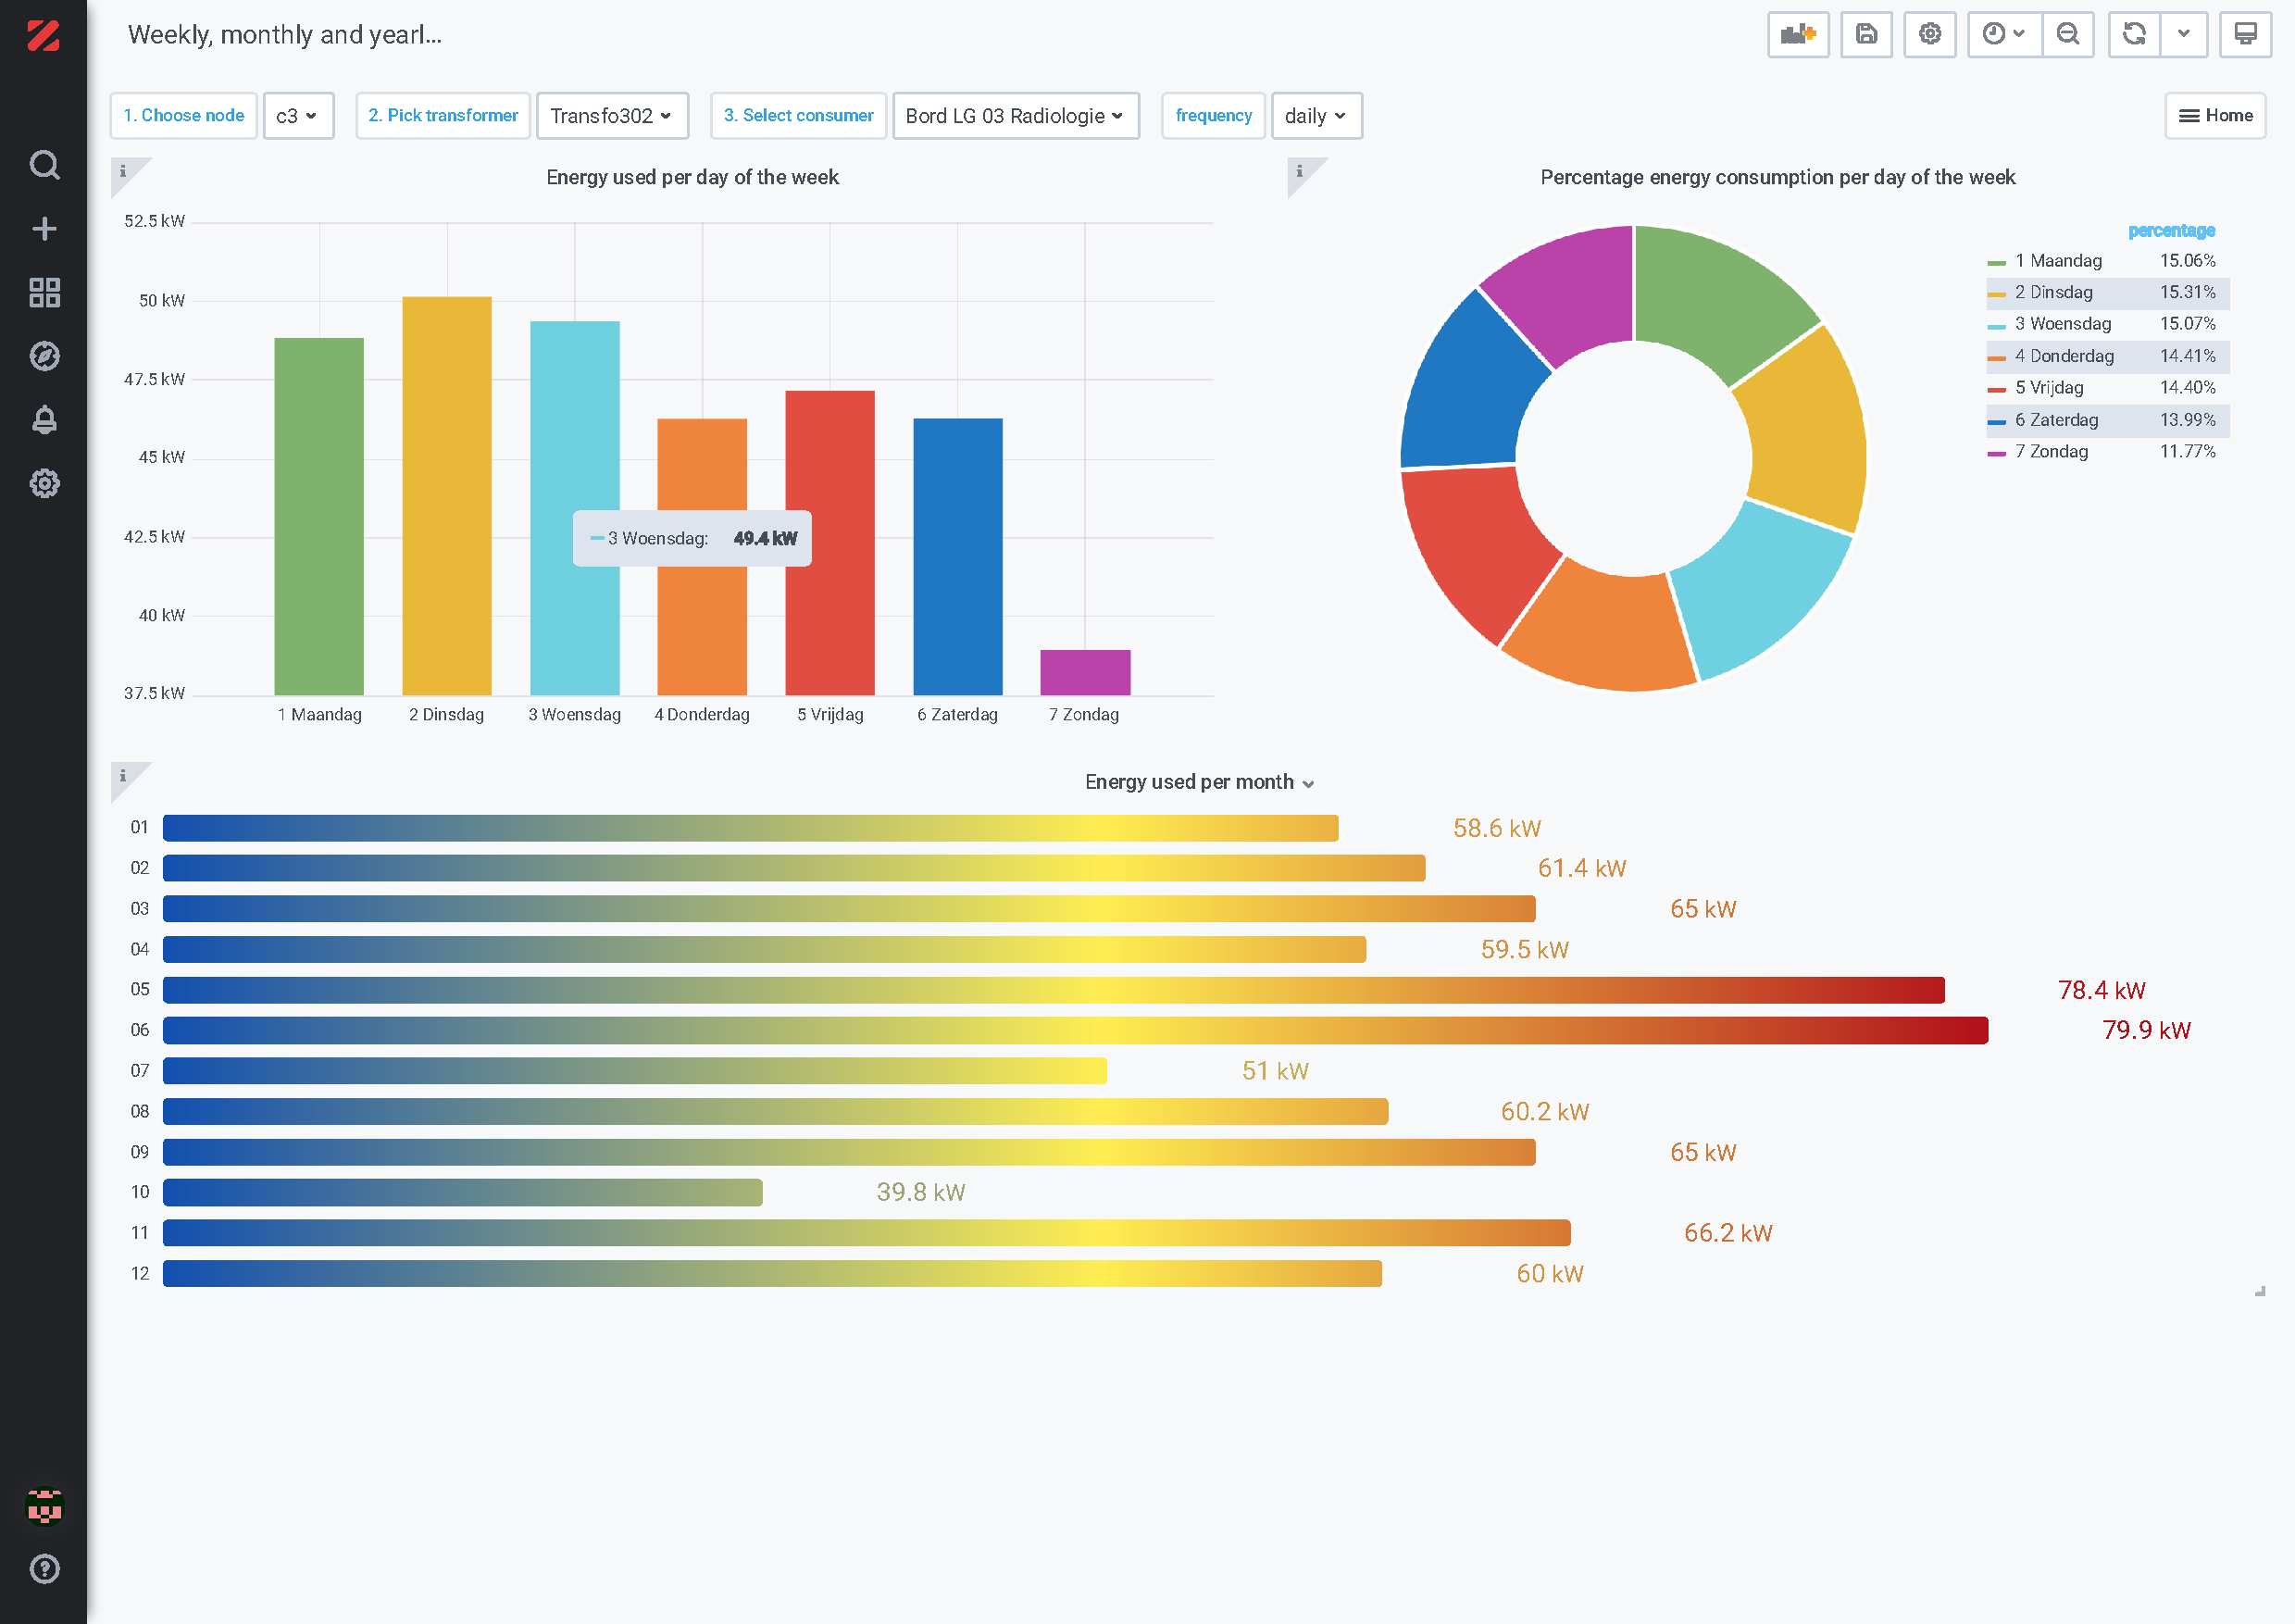
\includegraphics[clip, trim=0 5.5cm 0 0, width=\textwidth]{vub/grafana/weekly_and_monthly_node_c3_transfo302_radio.pdf}
        \caption{Per day of the week \& month}
        \label{fig:vub_stats_v2}
    \end{subfigure}
    \caption{Two examples of visualization dashboard of \ac{UZB} radiology's energy consumption}
    \label{fig:vub_2_dashboard}
\end{figure}

\subsection{Conclusion}
Concluding, we can state that \ac{VUB} researchers were fairly satisfied with the project result, as they now are able to monitor most of the hospital consumption via dashboards, in detail, everywhere through a web browser.
As evidence of this, they also decided to further expand the plan by adding a considerable amount of \ac{GEP} data, which became a separate sub-project.
% sextant \todo{EB: sicuro del ``sextant''?} No ho preso una cantonata.
However, potential enhancements remain open, such as additional statistics to compare nodes and viable alarms on current, voltage and power factor values. 




% \section{Climbing the information Ladder and difference between data and information}

% \section{Increase efficiency of tomato company}
% \textbf{21024}: Finally, I'd like to tell the tale of \cite{Misc:stoffels_en_website}:
% \begin{itemize}
%     \item how the demo of this project was launched with an intense daily sprint, followed by a duo collaboration with another inter;
%     \item how this project is a bit of a white fly compared to the zensor-standard project;
%     \item  was also an opportunity for me to test my skills in the role of backend rather than analysis.
% \end{itemize}
